\chapter{Prüfansätze}\label{cha:Pruefkonzepte}





Das nachfolgende Kapitel enthält Versuche und Überlegungen zu möglichen Messungen, um die im Kapitel~\ref{Eigenschaften_der_Aggregate} dargestellten Eigenschaften der Aggregate messtechnisch zu erfassen. Aus den Vorüberlegungen zu möglichen Tests für die NCAs (vgl. Kapitel~\ref{cha:Grundlagen_von_Pruefkonzepten_fuer_die_NCAs}) ergeben sich konkrete Prüfungen, die an NCAs auf dem derzeitigen Prüfstand im Rahmen dieser Arbeit versuchsweise durchgeführt werden. Denn wie in Kapitel~\ref{ch:Kritik_Testlauf} geäußert, reicht der derzeitige Testlauf nicht aus, um die verschiedenen Fehler beim Produktionsprozess der NCAs aufzudecken.



\section{Abfahren eines Profils unter Belastung}

Um die Belastungen der NCAs in der Produktion zu simulieren, können sie für die Testläufe extern belastet werden. Entweder kann die Achse auf Federn oder auf einen Block ausfahren oder es wird zur Belastung ein zusätzliches Gewicht an der Achse angebracht.



\subsection{Fahren auf eine Feder oder auf Block}\label{cha:Fahren auf eine Feder oder auf Block}


 
Eine Möglichkeit, viele Funktionen der NCAs auf einmal zu messen, ist, mit der Pinole der Achse auf eine Last zu fahren. Diese Art der Prüfung wird bereits bei der Erstmusterprüfung im Versuch praktiziert. Es kann entweder gegen Gasdruckfedern (vgl. Abbildung~\ref{fig:Fahren_auf_Feder}) oder auf Block (vgl. Abbildung~\ref{fig:Fahren_auf_Block}), d.h. gegen einen festen Widerstand (Metallklotz) gefahren werden. Mit dieser Messmethode kann sehr einfach überprüft werden, ob ein NCA die geforderten Kräfte aushalten kann.


%\colorbox{orange}{Bild einfügen}

\begin{figure}[H]
\centering
\begin{minipage}[b]{0.47\textwidth}
\centering
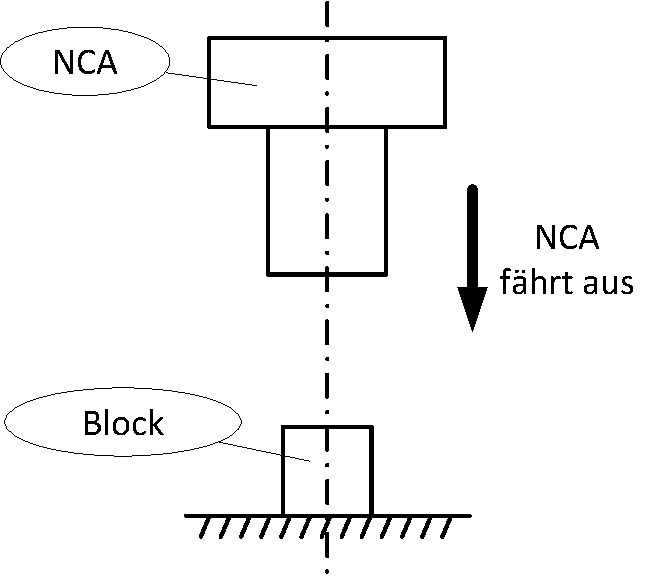
\includegraphics[width=\linewidth]{Fahren_auf_Block} 
\caption{Konzept: auf Block fahren} 
\label{fig:Fahren_auf_Block}
\end{minipage}
\begin{minipage}[b]{0.47\textwidth}
\centering
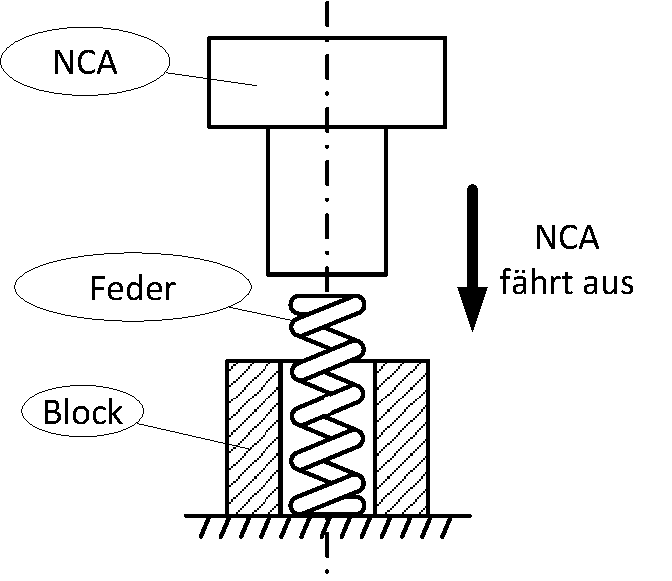
\includegraphics[width=\linewidth]{Fahren_auf_Feder} 
\caption{Konzept: Fahren auf eine Feder} 
\label{fig:Fahren_auf_Feder}
\end{minipage}

%\caption{Konzept Fahren auf Block und Feder}
%\label{fig:Fahren_auf_Block_und_Feder}
\end{figure}



Hierbei sind folgende Kriterien, die für oder gegen diese Messmethode im Serieneinsatz sprechen, abzuwägen:

Pro:
\begin{itemize}
 \item Statische Haltekräfte können nur auf diese Weise überprüft werden
 \item Entspricht einem realen Belastungsfall
 \item Absolute Positioniergenauigkeit und Wiederholgenauigkeit kann unter Belastung erfasst werden
\end{itemize}


Contra:
\begin{itemize}
 \item Hoher Aufwand
 \item Messung kann nicht ohne großen mechanischen Aufwand an anderen Maschinen als den Testmaschinen durchgeführt werden
  \item Arbeitssicherheit ist beim Testen schwer zu gewährleisten
  \item Belastungen können auch durch dynamische Kräfte abgebildet werden. Zur maximalen Auslastung des Aggregates ist das Fahren auf eine Last nicht erforderlich. (vgl.~\ref{cha:Polynom_5_Ordnung}) 
  \item Durch Schleppfehler kann das Spiel der Aggregate, auch ohne auf Belastung zu fahren, gemessen werden.
  \item Die absolute Positionierung des Aggregates (Positioniergenauigkeit) ist wesentlich stärker davon abhängig, ob auf Last gefahren wird, als die Wiederholgenauigkeit. Für den Einsatz ist die Wiederholgenauigkeit sehr viel wichtiger als die absolute Positioniergenauigkeit. 
  \item Es ist eine aufwendige Mechanik nötig, um verschiedene Hublängen messen zu können.
\end{itemize}

Als Fazit ergibt sich, dass man durch das Fahren auf Last nur wenige Erkenntnisse gewinnt, die man nicht auch auf andere Weise erlangen kann. Diese wenigen Erkenntnisse erfordern einen hohen Aufwand. Deshalb wird dieser Ansatz für die Umsetzung im Teststand für die Serienprüfung nicht weiter verfolgt.


% Der zusätzliche Gewinn an Erkenntnissen durch das Fahren auf Last wird durch die Gegenargumenten nicht gerechtfertigt.

\subsection{Anhängen eines Gewichtes oder einer Last}

Neben der Möglichkeit, mit der Achse auf eine Last zu fahren, kann auch durch das Anhängen einer Prüfmasse das Fahrverhalten verändert werden. Durch das veränderte Verhalten der Achse ist es möglich, neue Erkenntnisse zu gewinnen. Mit einem entsprechend hohen Gewicht kann man die Achse bis an ihre Grenzen belasten (siehe Abbildung~\ref{fig:NCA_mit_Zusatzgewicht}).

\begin{figure}[h]
\centering
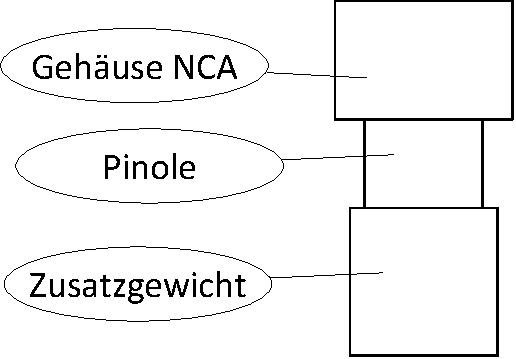
\includegraphics[width=0.4\textwidth]{NCA_mit_Zusatzgewicht} 
\caption{Konzept: Anhängen eines Zusatzgewichtes} 
\label{fig:NCA_mit_Zusatzgewicht}
\end{figure}



Wie aus Tabelle~\ref{tab:Traegheitsmoment_durch_Zusatzlast} ersichtlich, ändert diese Methode nur bei den kleinen NCAs wie den NCA 2 das Betriebsverhalten signifikant.

%Das Massenträgheitsmoment der Aggregate ohne Zusatzmasse ist der Übersichtstabelle der Aggregate von Riedle \cite{Riedle2015} zu entnehmen. Diese findet sich im Anhang~\ref{cha_Anhang_4}. Mit der bekannten Spindelsteigung $p$ und einem verwendeten zusätzlichen maximalen Gewicht von $m_{zus} = \SI{20}{\kilogram}$ ergeben sich die in der Tabelle~\ref{tab:Traegheitsmoment_durch_Zusatzlast} ersichtlichen Werte. Die \SI{20}{\kilogram} wurden nach dem Lastenhandhabungsgesetz abgeschätzt. Vergleiche Anhang~\ref{cha_Anhang_5}. Auch wirkt sich nach Formel~\ref{eq:Zusatzlast} die Zusatzmasse $m_{zus}$ bei großen Spindelsteigungen $p$ stärker aus als bei kleinen Gewindesteigungen.

Das Massenträgheitsmoment der Aggregate ohne Zusatzmasse ist der Übersichtstabelle der Aggregate von Riedle \cite{Riedle2015} zu entnehmen. Diese findet sich im Anhang~\ref{cha_Anhang_4}. Mit der bekannten Spindelsteigung $p$ und einem verwendeten zusätzlichen maximalen Gewicht von $m_{zus} = \SI{20}{\kilogram}$ laut Lastenhandhabungsgesetz (vgl. Anhang~\ref{cha_Anhang_5}) ergeben sich die aus der Tabelle~\ref{tab:Traegheitsmoment_durch_Zusatzlast} ersichtlichen Werte. So wirkt sich nach Formel~\ref{eq:Zusatzlast} die Zusatzmasse $m_{zus}$ bei großen Spindelsteigungen $p$ stärker aus als bei kleinen Gewindesteigungen.

%Die \SI{20}{\kilogram} wurden nach dem Lastenhandhabungsgesetz abgeschätzt. Vergleiche Anhang~\ref{cha_Anhang_5}.



\begin{equation}\label{eq:Zusatzlast}
J_{zus} = m_{zus} \cdot \left(\frac{p}{2 \cdot \pi}\right)^2
\end{equation}


\begin{table}[h]
\centering





\begin{tabular}{cccccc}\toprule
Aggregat Sach-Nr. & Aggregat & $p$ & $J_{NCA} $ & $J_{Zus.}$ & Unterschied \\
 &  & \si{\milli\meter} & \SI{e-6}{\kilogram\meter\squared} & \SI{e-6}{\kilogram\meter\squared} & \% \\
 \midrule
100-54-0590.0 & NCA 2 & 16 & 51 & 130 & 254 \\
100-54-0580.0 & NCA 2 & 5 & 42 & 13 & 30 \\
100-54-0592.0 & NCA 2 & 16 & 59 & 130 & 221 \\
100-54-0585.0 & NCA 2 & 16 & 46 & 130 & 283 \\
100-54-0575.0 & NCA 2 & 5 & 39 & 13 & 33 \\
100-54-0720.0 & NCA 3 & 10 & 352 & 51 & 14 \\
100-54-0730.0 & NCA 3 & 25 & 448 & 317 & 71 \\
100-54-0632.0 & NCA 4 & 16 & 1144 & 130 & 11 \\
100-54-0700.0 & NCA 4 & 10 & 1123 & 51 & 5 \\
100-54-0635.0 & NCA 5 & 15 & 4268 & 114 & 3 \\
100-54-0637.0 & NCA 5 & 10 & 4226 & 51 & 1 \\
\bottomrule
\end{tabular}
\caption{Trägheitsmoment durch eine Zusatzlast  $m_{zus}$ von \SI{20}{\kilogram}}
\label{tab:Traegheitsmoment_durch_Zusatzlast}
\end{table}





\section{Abfahren eines Profils im Leerlauf}\label{cha:Abfahren eines Profils im Leerlauf}



Neben der Möglichkeit auf Widerstände zu fahren oder die Achse mit einem Gewicht zu belasten, gibt es auch die Möglichkeit, die Achse im ``Leerlauf'' zu betreiben und so über den Zustand des NCAs Erkenntnisse zu gewinnen. Dabei versteht man unter Leerlauf laut Duden \textquote{das Laufen einer Maschine ohne Belastung} \cite{Duden_Leerlauf}, was in diesem Fall heißt, dass kein Werkzeug angebaut ist, das Arbeit verrichten könnte.

Um die Achsen mit der Steuerung betreiben zu können, müssen viele Daten generiert und verarbeitet werden, die zu einer Auswertung herangezogen werden können. Allerdings sind die meisten dieser Daten nur auf dem Regler vorhanden und können nicht in die VC 1 Steuerung übertragen werden. Mit dem Automation Studio, ein Softwaretools des Herstellers B\&R des Reglers, kann direkt auf dessen Daten zugegriffen werden. 

Dieser Zugriff ist allerdings aufwendig und kompliziert, da hierzu auf die Maschine über einen Fernwartungszugang zugegriffen werden muss. Außerdem ist dies risikoreich, weil mit dem Fernwartungszugang eine komplette Fernsteuerung der Maschine ermöglicht wird. Darüber hinaus können diese Testdaten während des derzeitigen Testablaufs nicht automatisiert erfasst werden. So bietet der direkte Zugriff auf die Daten des Reglers zwar eine Möglichkeit, auf diesem Weg gezielt viele, detaillierte Informationen zu gewinnen, wie es z.B. für die hier vorgestellten Untersuchungen nötig war. Aber man kann über den derzeit sehr aufwändigen und risikobehafteten Zugriff auf den Regler keine Standardmethode für die Erfassung der Daten der Testabläufe in der Serienproduktion entwickeln. Beispiele relevanter Messgrößen, die aus dem Regler ausgelesen werden können zeigt Tabelle~\ref{fig_Beispiele_relevanter_Daten_die_aus_dem_Regler_ausgelesen_werden_koennen}.


\begin{table}[H]
\center
\fbox{
\begin{minipage}[c]{0.6\textwidth}
\vspace{5pt}
\begin{itemize}
\item Positionen von Messlineal und Drehgeber
\item Stromstärke 
\item Drehmoment
\item Errechnete Reglerwerte wie z.B.
\begin{itemize}
\item Soll-Position
\item Sollgeschwindigkeit
\end{itemize}
\item Motortemperatur
\end{itemize}
\par\vspace{2pt}
\end{minipage}}
\caption{Aus dem Regler auslesbare Messgrößen}
\label{fig_Beispiele_relevanter_Daten_die_aus_dem_Regler_ausgelesen_werden_koennen}
\end{table}



Mit dem Automation Studio von B\&R können von den aus dem Regler ausgelesenen Daten sogenannte Traces aufgenommen werden. Dabei werden die ausgewählten Informationen mit einem eingestellten Zeitabstand über einen definierten Zeitbereich ausgelesen. Diese Informationen lassen sich abspeichern und auswerten. Manche dieser Werte (z.B. Stromstärke) werden zwar derzeit an die VC 1 Steuerung übergeben, können aber von dort aus dann nicht abgespeichert werden. 



%Deswegen weisen diese Aggregate ein anderes Fahrverhalten auf.

Neben dem Auslesen der Messgrößen aus dem Regler gibt es darüber hinaus  die Möglichkeit, weitere Messungen an den Aggregaten vorzunehmen, wie es bei den Tests in der Versuchsabteilung gemacht wird. Dafür werden u.a. beim Abfahren eines Profils im Leerlauf weitere Messungen wie z.B. Entfernungsmessungen mit Wirbelstromsensoren vorgenommen.

% Durch das Auslesen der Daten am Regler kann man viele Informationen über die NCAs gewinnen. Jedoch gibt es darüber hinaus die Möglichkeit, weitere Messungen an den Aggregaten vorzunehmen, wie es bei den Tests in der Versuchsabteilung gemacht wird. Dafür werden u.a. beim Abfahren eines Profils im Leerlauf weitere Messungen wie z.B. Entfernungsmessungen mit Wirbelstromsensoren vorgenommen.

Da eine der wichtigsten Funktionen der NCAs das positionsgenaue Abfahren einer Strecke ist, sind Messungen, die mit dem Fahrweg zusammenhängen, erwägenswert. Jedoch sind zusätzliche Wegmessung nur bei Aggregaten mit Ein-Geber-Regelung (vgl. Kapitel~\ref{cha_Steuerung_Aufbau_NCA}) sinnvoll. Bei der Zwei-Geber-Regelung (vgl. Kapitel~\ref{cha_Steuerung_Aufbau_NCA}) wird bereits ein direktes Wegmesssystem in Form eines Messlineals auf der Pinole eingesetzt. Eine zusätzliche Messung des Weges der Pinole würde nur die Genauigkeit des Messlineals überprüfen. Grobe Fehler beim Einbau des Messlineals könnten auch über die Vergleichsmessung mit dem Motorgeber erkannt werden.



Die Messungen beim Fahren im Leerlauf in diesem Kapitel werden an NCA 4 und NCA 5 durchgeführt, da diese eine Zwei-Geber-Regelung besitzen (vgl. Kapitel~\ref{cha:Unterschiede der NC-Aggregate}). Um Referenzwerte zu erhalten, werden alle zur Untersuchung genutzten Achsen mit den verschiedenen Fahrprofilen getestet.


% \subsection{Messunsicherheit bestimmen}
%\colorbox{orange}{Messunsicherheit einarbeiten?}

% Durch mehrmaliges Messen des gleichen Fahrprofil soll abgeklärt werden, wie stark die Werte innerhalb eines Aggregates schwanken, um zu wissen, wie groß die Abweichungen sind, wenn man nur wenige Messungen an anderen Aggregaten vornimmt. 

%Werte berechnen





\subsection{Langsames Abfahren im Trapezprofil}\label{cha:Langsames Abfahren im Trapezprofil}

Ein ähnliches Verfahren wird bereits im derzeitigen Testablauf verwendet. Wie in Kapitel \ref{ch:Ermittelte_Messwerte_Stromstaerke} beschrieben, wird die maximale Stromstärke im Bereich konstanter Geschwindigkeit gemessen. Das Fahrprofil wurde bereits in früheren Versuchen in der Versuchsabteilung entwickelt, um festzustellen, ob man damit eine Schwergängigkeit in bestimmten Bereichen der NCAs testen kann.

Mit dem Test des langsamen Abfahrens im Trapezprofil will man erkennen, ob das Aggregat beim Abfahren der maximal möglichen Strecke in bestimmten Streckenabschnitten schwergängiger ist als in anderen. Diese Schwergängigkeit erfordert ein erhöhtes Motormoment. Die Feststellung des erhöhten Momentes erfolgt indirekt über die Messung der Stromstärke. 

Wie bereits in Kapitel~\ref{cha:Asynchrone_Bewegung} beschrieben, gibt es aufgrund der Programmierung der VC 1 Steuerung nur die Möglichkeit, die Achsen im Asynchronbetrieb zu betreiben, wenn man sie mit einem trapezförmigen Geschwindigkeitsprofil fahren will. 


\begin{figure}[h]
\begin{tikzpicture}
\begin{groupplot}[
        group style={
            group size=1 by 2,
            xlabels at=edge bottom,
            ylabels at=edge left,
            xticklabels at=edge bottom,
            vertical sep=3pt,
            % vertical sep=40pt
        },
 	width=\textwidth,
 	xmin=0,
 	xmax=3.75,
 	%xtick={0,60,...,360},
 	xlabel={Zeit in \si{\second}},
    ]
    
    
    
\nextgroupplot [
 	no markers,
 	ymin=0,
    ymax=130,
  	%title=Einfahrzyklus Drehmomentprofil,
    ylabel={Position in \si{\milli\meter}},
    grid=major,
    ytick={0,20,...,120},
    height=0.25\textheight,
]
 	\addplot table[x=Zeit, y=Istpositionmm]  {graphen/CSV_Daten/Laufflaechenpruefung_1ne_Achse.txt};



\nextgroupplot [
 	no markers,
 	ymin=-5,
    ymax=5,
  	%title=Einfahrzyklus Drehmomentprofil,
    ylabel={Stromstärke in \si{\ampere}},
    grid=major,
    ytick={-5,-4,...,4},
    height=0.35\textheight,
]
 	\addplot table[x=Zeit, y=StromstaerkeA]  {graphen/CSV_Daten/Laufflaechenpruefung_1ne_Achse.txt};
\end{groupplot}
\end{tikzpicture}


\caption{Laufflächenprüfung einer Achse NCA4 $p=\num{10}$ mit der Seriennummer 38139}
\label{fig:Laufflaechenpruefung_einer_Achse}
\end{figure}

Um das Fahrprofil zu erstellen, werden in die VC 1 Steuerung des Teststandes für die Bewegung der Pinole die maximalen Beschleunigungen, die maximalen Geschwindigkeiten und die Endposition eingegeben. Während des Testlaufs wird der volle Hub des Aggregates mithilfe eines Trapezprofils (vgl. Kapitel \ref{cha:Asynchrone_Bewegung}) langsam abgefahren. Durch die im Vergleich zur Gesamtstrecke nur kurzen Beschleunigungsstrecken ist die Geschwindigkeit sehr lange konstant. (vgl. Abbildung~\ref{fig:Laufflaechenpruefung_einer_Achse}) 



Durch das langsame Abfahren wirken nur geringe Kräfte, vor allem Reibungskräfte sind hier zu erwähnen. Dies führt dazu, dass der Regler einen sehr starken Einfluss auf das Messergebnis hat, weil er ständig sehr stark nachregelt. Deshalb sind die Reglerauschläge sehr groß und es lässt sich nicht erkennen, ob die Ausschläge vom Regler selbst oder durch die Mechanik des NCAs verursacht wurden. Selbst mit weniger scharf eingestellten Reglerdaten ist eine aussagekräftige Messung nicht umsetzbar. 

%Einzelne Spitzenwerte sind als Messergebnis nicht zielführend, da sie zu sehr vom Regler beeinflusst werden. Als Alternative bietet es sich an, gemittelte Werte zu verwenden. Allerdings gehen einzelne nicht durch den Regler verursachte Ausschläge dann unter.

Dabei sind die dort ermittelten einzelnen Spitzenwerte als Messergebnis nicht aussagefähig, da sie zu sehr vom Regler beeinflusst werden. Als Alternative bietet es sich an, gemittelte Werte zu verwenden. Allerdings werden dann einzelne, nicht durch den Regler verursachte Ausschläge in den Mittelwert eingerechnet und können nicht der Schwergängigkeit zugeordnet werden.



  

Als Alternative wäre ein Fahrprofil denkbar, bei dem man eine Strecke mit konstantem Motorstrom abfährt. Die Schwergängigkeit könnte dann über den gemessenen Weg ermittelt werden.  Hierdurch könnte der Einfluss des Reglers vermindert werden. Dies ist aber aufgrund der derzeit verwendeten Steuerung  nicht umsetzbar. 

Bis jetzt ist das Problem der Schwergängigkeit in einzelnen Bereichen bei neuen NCAs noch nicht aufgefallen. Es ist davon auszugehen, dass die neuen NCAs leichtgängig sind, da sie während der Montage mehrfach von Hand gedreht werden müssen, um sie zu montieren. Gravierende Fehler werden deshalb bereits dort erkannt und direkt behoben. Dagegen kann es nach längerem Gebrauch zu einer Schwergängigkeit kommen. Eine Ursache hierfür könnte die ungleichmäßige Abnutzung sein, wenn die Achse immer nur in einem bestimmten kleineren Bereich hin- und hergefahren wird. Eine entsprechende Messung wäre daher bei einer regelmäßigen Wartung der NCAs sinnvoll, damit die Achsen nicht, wie derzeit üblich, erst nach einem Totalausfall zur Reparatur zurück zur Firma Bihler kommen.






\subsection{Abfahren im Stufenprofil}\label{cha:Abfahren im Stufenprofil}


Auch das Stufenprofil wurde bereits in der Versuchsabteilung der Firma Bihler entwickelt, um axiales Spiel erkennen zu können. Auf der Grundlage der bereits erarbeiteten Erkenntnisse soll die Tauglichkeit dieses Profils für die Prüfung der NCAs in der Serie überprüft werden. 

Durch kurzes, starkes Beschleunigen und Abbremsen kann hierbei ein hoher Ruck erzeugt werden. Wiederum soll, wie auch beim langsamen Abfahren (siehe Kapitel~\ref{cha:Langsames Abfahren im Trapezprofil}) ein Trapezprofil verwendet werden, weshalb die NCAs im Asynchronbetrieb laufen müssen. Um das Fahrprofil zu erstellen, werden auch wiederum in die VC 1 Steuerung des Teststandes für jeden einzelnen Bewegungsabschnitt der Pinole die maximalen Beschleunigungen, die maximalen Geschwindigkeiten und die Endposition eingegeben. Wie aus der Positionskurve in Abbildung \ref{fig:Axiales Spiel NCA 4 mit p = 10 und der Seriennummer 38147} ersichtlich, wird während der Ausfahrphase der Pinole an den Punkten 0, 30, 60, 90 und 120 mm stufenweise angehalten. Beim Einfahren wird an den Punkten 105, 75, 45, 15 angehalten, um dann wieder auf den Ausgangspunkt von 0 mm zu fahren. Es werden andere Punkte beim Einfahren angefahren als beim Ausfahren, um möglichst viele verschiedene Punkte des Fahrwegs abzudecken. An den Haltepunkten wird jeweils für einige Zeit in dieser Position verharrt bis zum nächsten Haltepunkt weitergefahren wird, damit das System genügend Zeit hat, sich wieder einzuschwingen. Eine kurze Verfahrstrecke von 30mm wird gewählt, um den Effekt öfter messen zu können und um das System einer starken Belastung zu unterziehen.


Insgesamt fährt somit die Pinole nicht, wie beim derzeitigen Testablauf, bis zu einem bestimmten Punkt aus und wieder ein, sondern sie fährt stufenweise, mit kurzen Beschleunigungs-, Brems- und Haltephasen komplett aus und wieder ein. Der Ruck wird sowohl beim Anfahren als auch beim Abbremsen erzeugt.
Um einen möglichst hohen Ruck zu erzeugen, wird so stark wie möglich beschleunigt und dann wieder abgebremst. 

Wie man aus dem Geschwindigkeitsprofil in Abbildung~\ref{fig:Axiales Spiel NCA 4 mit p = 10 und der Seriennummer 38147}~B erkennt, wird durch die kurzen Verfahrstrecken und die vorgegebene maximale Beschleunigung aus dem Trapezprofil annähernd ein Dreiecksprofil. Die erreichte maximale Geschwindigkeit ist wegen des kurzen Fahrweges kleiner als die Geschwindigkeit, die das Aggregat maximal fahren kann. Eine Fahrstrecke mit konstanter Geschwindigkeit ohne Beschleunigung, wie sie beim Trapezprofil ansonsten gefahren wird, ergibt sich hier nicht. Wie bereits in Kapitel~\ref{ch:Ermittelte_Messwerte_Stromstaerke} beschrieben, ist die in Abbildung~\ref{fig:Axiales Spiel NCA 4 mit p = 10 und der Seriennummer 38147}~C dargestellte Drehmomentkurve der Beschleunigungskurve annähernd gleichzusetzen. 

% Auch die Drehmomentkurve ist in der Abbildung~\ref{fig:Axiales Spiel NCA 4 mit p = 10 und der Seriennummer 38147}~C zu sehen. 

Nachdem im Fahrprofil die maximalen Beschleunigungen, die maximalen Geschwindigkeiten und die Endposition festgelegt werden, ergeben sich die Kurven für die Geschwindigkeit und das Drehmoment in Abbildung \ref{fig:Axiales Spiel NCA 4 mit p = 10 und der Seriennummer 38147} aus den Ableitungen der Positionskurve.

\clearpage

\begin{figure}[H]
\centering
\begin{tikzpicture}
\begin{groupplot}[
        group style={
            group size=1 by 5,
            xlabels at=edge bottom,
            ylabels at=edge left,
            xticklabels at=edge bottom,
            vertical sep=3pt,
            % vertical sep=40pt
        },
 	width=\textwidth,
 	xmin=0,
 	xmax=1.25,
 	xtick={0,0.1,...,1.2},
 	xlabel={Zeit in $s$},
 	yticklabel style = {font=\small,xshift=0.25ex},
 	,
 	ylabel style = {font=\small,xshift=0.25ex},
    ]
    
\nextgroupplot [
 	no markers,
 	ymin=0,
    %ymax=5,
  	%title=Einfahrzyklus Drehmomentprofil,
    ylabel={Position in \si{\milli\meter}},
    grid=major,
    ytick={0,15,...,120},
    height=0.23\textheight,
]
    
 	\addplot table[x=Zeit, y=Position]  {graphen/CSV_Daten/Axiales_Spiel_1-10788-38147-A-29.05.2015-p10.txt};
 	\node[anchor=center] at (axis cs:1.15,105) {A};
    
\nextgroupplot [
 	no markers,
 	%ymin=0,
    %ymax=130,
  	%title=Einfahrzyklus Drehmomentprofil,
    ylabel={Geschwindigkeit in \si{\per\second}},
    grid=major,
    ytick={-75,-50,...,75},
    height=0.23\textheight,
]
 	\addplot table[x=Zeit, y=Geschwindigkeit]  {graphen/CSV_Daten/Axiales_Spiel_1-10788-38147-A-29.05.2015-p10.txt};
 	\node[anchor=center] at (axis cs:1.15,60) {B};


\nextgroupplot [
 	no markers,
 	%ymin=0,
    %ymax=130,
  	%title=Einfahrzyklus Drehmomentprofil,
    ylabel={Drehmoment in \si{\newton\meter}},
    grid=major,
    %ytick={0,20,...,120},
    height=0.23\textheight,
]
 	\addplot table[x=Zeit, y=Drehmoment]  {graphen/CSV_Daten/Axiales_Spiel_1-10788-38147-A-29.05.2015-p10.txt};
 	\node[anchor=center] at (axis cs:1.15,20) {C};

\nextgroupplot [
 	no markers,
 	ymin=-0.05,
    ymax=0.05,
  	%title=Einfahrzyklus Drehmomentprofil,
    ylabel={Schleppfehler in \si{\milli\meter}},
    grid=major,
    %ytick={0,20,...,120},
    height=0.23\textheight,
    scaled y ticks = false,
    tick label style={/pgf/number format/fixed},
]
 	\addplot table[x=Zeit, y=Lag_error]  {graphen/CSV_Daten/Axiales_Spiel_1-10788-38147-A-29.05.2015-p10.txt};
 	\node[anchor=center] at (axis cs:1.15,0.025) {D};
 	
 	
\nextgroupplot [,
 	no markers,
 	ymin=-0.1,
    ymax=0.1,
  	%title=Einfahrzyklus Drehmomentprofil,
    ylabel={Positionsdifferenz in \si{\milli\meter}},
    grid=major,
    %ytick={0,20,...,120},
    height=0.23\textheight,
    scaled y ticks = false,
    tick label style={/pgf/number format/fixed},
]
 	\addplot table[x=Zeit, y=Position_difference]  {graphen/CSV_Daten/Axiales_Spiel_1-10788-38147-A-29.05.2015-p10.txt};
 	\node[anchor=center] at (axis cs:1.15,0.075) {E};

\end{groupplot}

%\draw (my plots c1r1.east) circle (3pt) node {East};


\end{tikzpicture}
\caption{Kennkurven (A bis E) des Stufenprofiles eines  NCA 4 mit p = 10 und der Seriennummer 38147}
\label{fig:Axiales Spiel NCA 4 mit p = 10 und der Seriennummer 38147}
\end{figure}


\subsubsection{Messgrößen}\label{cha: Messgroessen Stufenprofil}


Durch die auftretenden hohen Rucke im Fahrprofil Stufenprofil wirkt sich ein eventuell vorhandenes Spiel der Bauteile besonders stark auf das Fahrverhalten der Achse aus. Neben der Mechanik der einzelnen Aggregate beeinflusst auch der Regler das Fahrverhalten sehr stark. Ein idealer Regler sollte unabhängig von der Regelstrecke ein immer gleiches Fahrprofil erzeugen. Somit ist es zur Messung erforderlich, Messgrößen zu finden, bei denen die Auswirkungen von Unstimmigkeiten in der Mechanik besonders deutlich sichtbar werden. Aus diesem Grund bieten sich insbesondere die  Messgrößen Positionsdifferenz und Schleppfehler an.

Unter Schleppfehler (Lag error) versteht man den Unterschied zwischen der vom Regler gesetzten Position (Soll-Position) und der durch das Messlineal erfassten tatsächlichen Position (Ist-Position). Er ist auch unter dem Begriff Regeldifferenz bekannt. Diesen Schleppfehler versucht der Regler ständig auf Null zu reduzieren. Besonders bei Be- und Entschleunigungsvorgängen entsteht ein großer Schleppfehler (vgl. Abbildung~\ref{fig:Axiales Spiel NCA 4 mit p = 10 und der Seriennummer 38147}~D).


%Die Abweichung der Soll-Position von der Ist-Position kann entweder durch Fehler (z.B. axiales Spiel) oder durch Elastizitäts- und Trägheitseffekte herrühren. Bei 

Unter der Positionsdifferenz (Positions difference) ist die Differenz zwischen der aktuellen Position des Motorgebers und der aktuellen Position des Messlineals zu verstehen, die nur bei einem Aggregat mit einem 2-Geber-System gemessen werden kann (vgl. Kapitel~\ref{cha:Unterschiede der NC-Aggregate}). Durch Temperatur, Steigungsfehler oder Nachgiebigkeit der Bauteile weichen die beiden Positionen im Normalbetrieb voneinander ab. Beispielhaft ist der Verlauf der Positionsdifferenz in Abbildung~\ref{fig:Axiales Spiel NCA 4 mit p = 10 und der Seriennummer 38147}~E zu sehen. % Durch Temperatureinflüsse verändert sich diese Kurve während des Betriebes.

Die Positionsdifferenz-Kurve wird durch die Temperatur beeinflusst.  Eine Temperaturerhöhung führt z.B. zu einer Längenzunahme der Spindel des Gewinderollentriebes. Durch die veränderte Länge der Spindel verändert sich auch die Steigung der Spindel leicht. Somit wird für den gleichen axialen Weg eine geringere Drehbewegung benötigt. 


Je länger die Achse betrieben wird, desto höher wird die Temperatur in der Achse. Da die Positionsdifferenz-Kurve durch die Temperatur und somit die Laufzeit beeinflusst ist, liegen hier die Kurven nicht identisch übereinander, sondern sind verschoben und verzerrt.




\subsubsection{Mittelwerte und Kennwerte der NC-Aggregate}\label{cha:Mittelwerte und Kennwerte der NC-Aggragate}

Nach dem in der Firma üblichen Testzyklus, der im Kapitel~\ref{cha:Bisheriger Testablauf} beschrieben ist, werden 19 neue, aufgrund des Testlaufs eingefahrene NCA 4 mit der Steigung $p = 10$ (Artikelnummer: 100-54-0700.0) auf dem Teststand mit dem Stufenprofil betrieben, um Erkenntnisse zu gewinnen, ob dies eine aussagekräftige Testmethode ist. Während des Fahrens werden von jedem NCA dreimal hintereinander Traceaufnahmen der Kennlinien aufgenommen, sodass man pro Achse drei verschiedene Traces erhält. Bei der Auswertung der Messungen ergibt sich, dass die Kennlinien sehr ähnlich verlaufen. Bei den ausgewerteten Kennlinien handelt es sich um Kennlinien von der Positionsdifferenz, des Schleppfehlers, des Drehmoments und als Vergleichsbasis der Soll-Position.

Wie bereits in Kapitel~\ref{cha: Messgroessen Stufenprofil} beschrieben, ändert sich die Kennkurve der Positionsdiffernz bei sich verändernden Temperaturen. Aus diesem Grund ist diese Kennkurve bei unterschiedlichen Messungen verschoben und verzerrt.


Da die Kennlinien der verschiedenen Parameter bei den im Stufenmodell gefahrenen NCA 4 sehr ähnlich verlaufen, kann man davon ausgehen, dass es sich um die Standardwerte störungsfreier NCA 4 handelt. Um für zukünftige Messungen Referenzkurven zu besitzen, werden aus den gemessenen Werten neue Kurven mit den Mittelwerten der einzelnen Kurvenpunkte generiert und als Kennlinien verwendet. 


So ist zu vermuten, dass Abweichungen von diesen Kennlinien auf Fehler der NCAs zurückzuführen sind. Diese Fehler können entweder dadurch verursacht sein, dass es Probleme mit der Steuerung gibt, oder dass die Achse selbst eine Funktionsstörung aufweist.






\subsubsection{Erkennen von axialem Spiel} \label{cha:Fehlerermittlung von axialem Spiel Stufenprofil}

Alle 19 NCA 4, die zum Testen mithilfe des Stufenprofils zur Verfügung stehen, weisen bei dem Absolvieren des bisherigen Testablaufs (vgl. Kapitel~\ref{cha:Bisheriger Testablauf}) keinerlei Auffälligkeiten auf.

Bei der nachfolgenden Erstellung der Kennwertkurven für Schleppfehler und Positionsdifferenz ergibt das Abfahren des Stufenprofils sehr ähnliche Kurvenverläufe nur für 18 der 19 getesten NCA 4.

\begin{figure}[H]
\centering




\begin{tikzpicture}
\begin{groupplot}[
        group style={
            group size=1 by 2,
            xlabels at=edge bottom,
            ylabels at=edge left,
            xticklabels at=edge bottom,
            vertical sep=3pt,
            % vertical sep=40pt
        },
 	width=\textwidth,
 	xmin=0,
 	xmax=1.25,
 	xtick={0,0.1,...,1.2},
 	xlabel={Zeit in \si{\second}},
 	yticklabel style = {font=\small,xshift=0.25ex},
 	,
 	ylabel style = {font=\small,xshift=0.25ex},
    ]
    
\nextgroupplot [
 	no markers,
 	%ymin=-0.05,
    %ymax=0.05,
  	%title=Einfahrzyklus Drehmomentprofil,
    ylabel={Schleppfehler in \si{\milli\meter}},
    grid=major,
    %ytick={0,20,...,120},
    height=0.3\textheight,
    scaled y ticks = false,
    tick label style={/pgf/number format/fixed},
]
    \addplot table[x=Zeit, y=MittelwertLagError]  {graphen/CSV_Daten/zusammengefasst_axiales_Spiel.txt};
 	\addplot table[x=Zeit, y=lag_error]  {graphen/CSV_Daten/Zu_viel_Axiales_Spiel_1-10788-38173-A-16.06.2015-p10.txt};
 	\addplot[lightgray,very thin] table[x=Zeit, y=minus3sigmaMittelwertLagError]  {graphen/CSV_Daten/zusammengefasst_axiales_Spiel.txt};
 	\addplot[lightgray,very thin] table[x=Zeit, y=plus3sigmaMittelwertLagError]  {graphen/CSV_Daten/zusammengefasst_axiales_Spiel.txt};
 	\node[anchor=center] at (axis cs:1.15,0.06) {A};
 	
\nextgroupplot [
 	no markers,
 	%ymin=-0.1,
    %ymax=0.1,
  	%title=Einfahrzyklus Drehmomentprofil,
    ylabel={Positionsdifferenz in \si{\milli\meter}},
    grid=major,
    %ytick={0,20,...,120},
    height=0.3\textheight,
    scaled y ticks = false,
    tick label style={/pgf/number format/fixed},
    legend entries={Mittelwert aller Achsen, zu viel Spiel Sn.: 38173, $\pm 3 \sigma $ Standardabweichung},
]
 	\addplot table[x=Zeit, y=MittelwertPositionsDifference]  {graphen/CSV_Daten/zusammengefasst_axiales_Spiel.txt};
 	\addplot table[x=Zeit, y=Positions_Differenz]  {graphen/CSV_Daten/Zu_viel_Axiales_Spiel_1-10788-38173-A-16.06.2015-p10.txt};
 	\addplot[lightgray,very thin] table[x=Zeit, y=minus3sigmaPositionsDifference]  {graphen/CSV_Daten/zusammengefasst_axiales_Spiel.txt};
 	\addplot[lightgray,very thin] table[x=Zeit, y=plus3sigmaPositionsDifference]  {graphen/CSV_Daten/zusammengefasst_axiales_Spiel.txt};
 	\node[anchor=center] at (axis cs:1.15,0.04) {B};

\end{groupplot}
\end{tikzpicture}
\caption{Vergleich von Mittelwert aller Achsen und Achse mit axialem Spiel im Stufenprofil}
\label{fig:Vergleich von Mittelwert und Achse mit axialem Spiel}
\end{figure}



Wie der Abbildung~\ref{fig:Vergleich von Mittelwert und Achse mit axialem Spiel} entnommen werden kann, weicht der Kurvenverlauf des NCA mit der Seriennummer 38173 sowohl beim Schleppfehler (Abbildung~\ref{fig:Vergleich von Mittelwert und Achse mit axialem Spiel} A) als auch bei der Po\-si\-tions\-dif\-fe\-renz (Abbildung~\ref{fig:Vergleich von Mittelwert und Achse mit axialem Spiel} B) signifikant von der Mittellinie aller fast übereinstimmenden anderen Kurven ab. Zudem sind bei keiner der anderen Kurven die Ausschläge des Schleppfehlers und der Positionsdifferenz beim Ausfahren (Zeit von 0 bis 0,55 Sekunden) annähernd so groß wie bei dieser Achse. Beim Einfahren (Zeit von 0,55 bis 1,2 Sekunden) sind keine größeren Abweichungen vom Mittelwert aller anderen Achsen erkennbar.



Um dieser Unstimmigkeit auf den Grund zu gehen, wird die Achse demontiert. Bei der Demontage des Aggregates wird festgestellt, dass die Abstimmscheibe 0,03 mm Spiel verursacht und nicht, wie eigentlich vorgesehen, 0,03 - 0,05 mm Vorspannung erzeugt. Somit ist die Abstimmscheibe um mindestens 0,06 mm zu klein abgestimmt worden. Dies hat zur Folge, dass in axialer Richtung axiales Spiel vorhanden ist, sodass die Kopplung von radialer Motorbewegung zeitweise nicht mehr direkt in eine Axialbewegung der Pinole umgesetzt wird. Die verschiedenen möglichen Entstehungstellen von axialem Spiel sind der Abbildung~\ref{fig:Entstehungstellen von Axialem Spiel} zu entnehmen.


\begin{figure}[H]
\centering
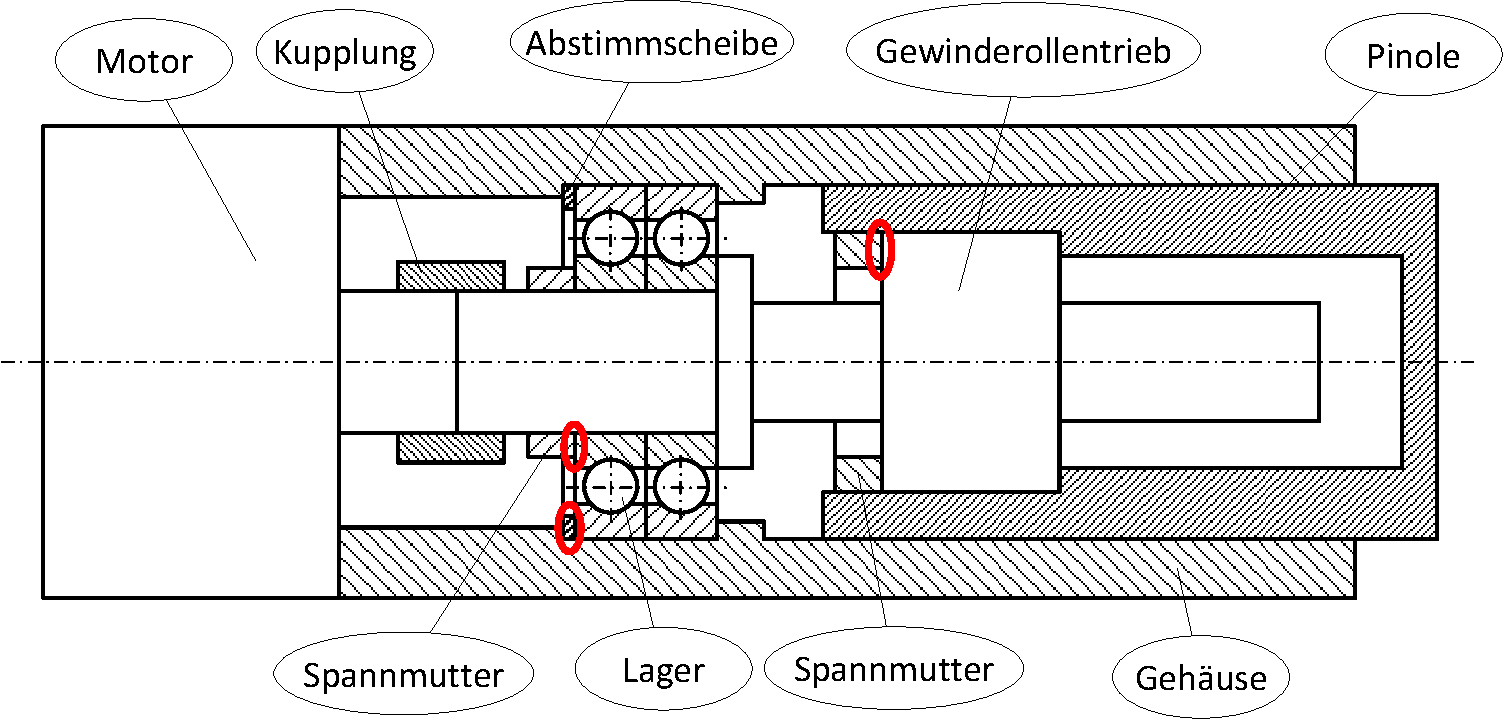
\includegraphics[width=0.9\textwidth]{NC_Aggregat_Skizze1_mit_Beschriftung_axiales_Spiel}
\caption{Mögliche Entstehungsstellen von axialem Spiel}
\label{fig:Entstehungstellen von Axialem Spiel}
\end{figure}

%Vor der Demontage wird die Achse einmal um \SI{180}{\degree} gedreht, sodass die Pinole senkrecht nach oben zeigt, und nicht wie bei dem sonstigen Testablauf senkrecht nach unten. In dieser Position wird dasselbe Stufenprofil erneut gefahren. Bei den erneut gemessenen Kennlinien zeigt sich, dass die Abweichung von den Mittelwerten nun während der Einfahrtphase der Pinole zu erkennen ist und die Ausfahrtphase keine größeren Abweichungen aufweist. Als mögliche Erklärung kommt in Frage, dass die Gravitationskraft der Erde dafür verantwortlich ist, dass das Spiel in Abbildung~\ref{fig:Vergleich von Mittelwert und Achse mit axialem Spiel} nur während des Ausfahrens (Zeit von 0 bis 0,55 Sekunden) zu erkennen ist. Die entsprechenden Referenzprofile sind im Anhang~\ref{cha:Anhang_3} zu finden.

%Um das axiale Spiel mit dem Fahren im Stufenprofil deutlich zu erkennen, sollten die Achsen nach den bisherigen Erkenntnissen senkrecht montiert sein.







Nach der Demontage wird das Aggregat mit einer passenden Abstimmscheibe wieder montiert. Bei einem anschließenden erneuten Testlauf mit dem Stufenprofil weisen die Kennkurven keine Besonderheiten mehr auf. Somit ist davon auszugehen, dass die starke Abweichung von der Mittelwertkennlinie auf die falsch abgestimmte Abstimmscheibe zurückzuführen sind.

Mit dem Verfahrprofil Stufenprofil kann aufgrund der hohen Rücke axiales Spiel erkannt werden. Es wäre möglich, dieses Profil in einen erweiterten Testablauf zu integrieren.

Allerdings wurde die Praxistauglichkeit dieser Messmethode nur beispielhaft an dem Aggregattyp NCA 4 $p = 10$ (Artikelnummer 100-54-0700.0) durchgeführt. Für alle anderen Aggregattypen müssten noch Referenzprofile ermittelt werden. 




\subsubsection{Messung mit und gegen Gravitation}\label{cha:Anhang_3}


Die Achse mit axialem Spiel wird mit dem gleichem Zyklus einmal mit der Gravitaionskraft und einmal gegen die Gravitationskraft betrieben. Als Vergleichswert wird die Achse nach dem Abstimmen ohne axiales Spiel gefahren. 

So wird die Achse vor der Demontage einmal um \SI{180}{\degree} gedreht, sodass die Pinole senkrecht nach oben zeigt, und nicht wie bei dem sonstigen Testablauf senkrecht nach unten. In dieser Position wird dasselbe Stufenprofil erneut gefahren. Bei den erneut gemessenen Kennlinien zeigt sich, dass die Abweichung von den Mittelwerten nun während der Einfahrtphase der Pinole zu erkennen ist und die Ausfahrtphase keine größeren Abweichungen aufweist. Als mögliche Erklärung kommt in Frage, dass die Gravitationskraft der Erde dafür verantwortlich ist, dass das Spiel in Abbildung~\ref{fig:Vergleich von Mittelwert und Achse mit axialem Spiel} nur während des Ausfahrens (Zeit von 0 bis 0,55 Sekunden) zu erkennen ist. Die entsprechenden Profile sind in Abbildung~\ref{fig_Mit_Gravitation} zu finden.


\begin{figure}[H]
\centering




\begin{tikzpicture}
\begin{groupplot}[
        group style={
            group size=1 by 2,
            xlabels at=edge bottom,
            ylabels at=edge left,
            xticklabels at=edge bottom,
            vertical sep=3pt,
            % vertical sep=40pt
        },
 	width=0.9\textwidth,
 	xmin=0,
 	xmax=1.25,
 	xtick={0,0.1,...,1.3},
 	xlabel={Zeit in \si{\second}},
 	yticklabel style = {font=\small,xshift=0.25ex},
 	,
 	ylabel style = {font=\small,xshift=0.25ex},
    ]
    
\nextgroupplot [
 	no markers,
 	%ymin=-0.05,
    %ymax=0.05,
  	%title=Einfahrzyklus Drehmomentprofil,
    ylabel={Schleppfehler in \si{\milli\meter}},
    grid=major,
    %ytick={0,20,...,120},
    height=0.3\textheight,
    scaled y ticks = false,
    tick label style={/pgf/number format/fixed},
]
 	\addplot table[x=Zeit, y=Lag_error]  {graphen/CSV_Daten/Axiales_Spiel_3-10788-38173-A-stehend.txt};
 	\addplot table[x=Zeit, y=Lag_error]  {graphen/CSV_Daten/Axiales_Spiel_3-10788-38173-A-andereRichtung.txt};
 	\addplot table[x=Zeit, y=Lag_error]  {graphen/CSV_Daten/Axiales_Spiel_3-10788-38173-A-ohne_Spiel.txt};
 	\node[anchor=center] at (axis cs:1.15,0.06) {A};
 	
\nextgroupplot [
 	no markers,
 	%ymin=-0.1,
    %ymax=0.1,
  	%title=Einfahrzyklus Drehmomentprofil,
    ylabel={Positionsdifferenz in \si{\milli\meter}},
    grid=major,
    %ytick={0,20,...,120},
    height=0.3\textheight,
    scaled y ticks = false,
    tick label style={/pgf/number format/fixed},
    legend entries={Ausfahren mit Graviatation, Ausfahren gegen Graviatation, ohne Spiel},
]
 	\addplot table[x=Zeit, y=Position_difference]  {graphen/CSV_Daten/Axiales_Spiel_3-10788-38173-A-stehend.txt};
 	\addplot table[x=Zeit, y=Position_difference]  {graphen/CSV_Daten/Axiales_Spiel_3-10788-38173-A-andereRichtung.txt};
 	\addplot table[x=Zeit, y=Position_difference]  {graphen/CSV_Daten/Axiales_Spiel_3-10788-38173-A-ohne_Spiel.txt};
 	\node[anchor=center] at (axis cs:1.15,0.03) {B};

\end{groupplot}
\end{tikzpicture}
\caption{Mit Gravitation, gegen Gravitation und ohne Spiel, NCA 4 p=10 Seriennummer 38173}
\label{fig_Mit_Gravitation}
\end{figure}


Um das axiale Spiel mit dem Fahren im Stufenprofil deutlich zu erkennen, sollten die Achsen nach den bisherigen Erkenntnissen senkrecht montiert sein.

%Die Achse mit axialem Spiel wird mit dem gleichem Zyklus einmal mit und einmal gegen die Gravitationskraft betrieben. Als Vergleichswert wird die Achse nach dem Abstimmen ohne Aaiales Spiel dargestellt.







\subsection{Abfahren im Maximalprofil Polynom 5. Ordnung} \label{cha:Polynom_5_Ordnung}



Die Relativbewegung von 2 Getriebegliedern kann außer mit dem Trapezprofil auch mit der analytischen Funktion Polynom 5. Ordnung beschrieben werden. Da das Bewegungsgesetz Polynom 5. Ordnung vielseitig anwendbar ist, wird es in der Praxis vielfach genutzt~\cite{Braune2009a}. Es ist auch bei der Steuerung der NCAs der Firma Bihler das am häufigsten eingesetzte Bewegungsgesetz. Deshalb bietet es sich an, zu analysieren, ob beim Testen der NCAs nach der Funktion Polynom 5.~Ordnung Fehler entdeckt werden können.

Nachdem Fehler am häufigsten unter hoher Belastung auftreten, muss das Fahrprofil so programmiert werden, dass die Aggregate mit höchst möglicher Beschleunigung und Geschwindigkeit gefahren werden.

\subsubsection{Berechnung des Fahrprofils}

Um eine möglichst hohe Beschleunigung und Geschwindigkeit zu erreichen,  müssen eine Strecke und eine Zeit für die Eingabe in die Steuerung berechnet werden. Bei dieser Berechnung des Profils werden als Eingangsparameter die zulässige maximale Geschwindigkeit und die maximale Beschleunigung des jeweiligen Aggregates verwendet. Diese können der Übersichtstabelle der NCAs \cite{Riedle2015} entnommen werden. Bei manchen Aggregaten erzeugt die laut Tabelle angegebene Beschleunigung ein Moment, das größer ist als das, das der Motor erzeugen kann. Entsprechend muss erst die maximal größte Beschleunigung nach Gleichung~\ref{eq:max beschleunigung} berechnet werden.



\begin{equation}\label{eq:max beschleunigung}
\dot{n}_{\mathrm{NCA, max}} = \frac{M_{\mathrm{NCA, max}}}{J_{NCA} \cdot 2 \cdot \pi}
\end{equation}


Die Berechnung erfolgt auf Basis der VDI-Richtlinie 2143 \cite{VDI2002}. Als Übergangsbedingung wird hier der Übergang Rast-in-Rast gewählt. 

Das normierte Bewegungsgesetz für Rast-in-Rast (R-R) mit dem Polynom 5. Ordnung lautet:

\begin{align}
f(z) &= 10 \cdot z^3 - 15 \cdot z^4 + 6 \cdot z^5 \\
f'(z) &= 30 \cdot z^2 - 60 \cdot z^3 + 30 \cdot z^4 \\
f''(z) &= 60 \cdot z - 180 \cdot z^2 + 120 \cdot z^3 
\end{align}





Durch den Drehgeber der Maschine ist die Winkelgeschwindigkeit des Kurvenkörpers konstant:

\begin{equation}\label{eq:2}
\dot{\varphi} = \mathrm{konstant}
\end{equation}

Hieraus ergibt sich für die Abtriebsgeschwindigkeit und die Abtriebsbeschleunigung für ein gerade geführtes Abtriebsglied:



\begin{align}
\dot{s} &= s' \cdot \dot{\varphi}  \label{eq:Abtriebsgeschwindigkeit}\\
\ddot{s} &= s'' \cdot {\dot{\varphi}}^2 \label{eq:Abtriebsbeschleunigung}
\end{align}







% \subsubsection{Berechnung für die Geschwindigkeit}



Um als Erstes die Bewegungsgleichung der Abtriebsgeschwindigkeit~\ref{eq:Abtriebsgeschwindigkeit} nach $n_{\mathrm{Ma, max}}$ aufzulösen, wird zunächst die Gleichung~\ref{eq:Abtriebsgeschwindigkeit} für einen einzelnen Bewegungsabschnitt $\mathrm{ik}$ definiert:


% Als erstes wird die Bewegungsgleichung der Abtriebsgeschwindigkeit~\ref{eq:Abtriebsgeschwindigkeit} nach $n_{\mathrm{Ma, max}}$ aufgelöst. Hierfür wird die Gleichung~\ref{eq:Abtriebsgeschwindigkeit} für einen einzelnen Bewegungsabschnitt $\mathrm{ik}$ definiert:

\begin{equation}
\dot{s}_{\mathrm{ik}} = s'_{\mathrm{ik}} \cdot \dot{\varphi}
\end{equation}

Mit $\dot{\varphi}  = 2 \cdot \pi \cdot  n_{\mathrm{Ma, max}} $ und der Übertragungsfunktion 1. Ordnung $s'_{\mathrm{ik}} = f'_{\mathrm{ik}}(z) \cdot \frac{180}{\pi} \cdot \frac{S_{\mathrm{ik}}}{\Phi_{\mathrm{ik}}}$ folgt:

\begin{equation}\label{eq:1}
\dot{s}_\mathrm{ik}  = f'_\mathrm{ik}(z) \cdot 360 \cdot \frac{S_{\mathrm{ik}}}{\Phi_{\mathrm{ik}}} \cdot  n_{\mathrm{Ma, max}}
\end{equation}

Die Geschwindigkeit des Abtriebgliedes $\dot{s}$ kann durch die bekannten Größen (vgl. \cite{Riedle2015}) Steigung des Gewinderolltriebes $p$ und die maximale Drehzahl des Aggregates $n_{\mathrm{NCA, max}}$ wie folgt dargestellt werden:

\begin{equation}
\dot{s} =p \cdot n_{\mathrm{NCA, max}}
\end{equation}


Des Weiteren wird die 1. Ableitung des Bewegungsgesetzes $f'(z)$ für $z = 0.5$ maximal. Dies ergibt den Wert $f'(0.5)= \frac{15}{8}$. In die Gleichung~\ref{eq:1} eingesetzt ergibt sich:

\begin{equation}
p \cdot n_{\mathrm{NCA, max}} = 675 \cdot \frac{S_{\mathrm{ik}}}{\Phi_{\mathrm{ik}}} \cdot  n_{\mathrm{Ma, max}}
\end{equation}



Nach der maximalen Drehzahl der Maschine $n_{\mathrm{Ma, max}}$ aufgelöst, ergibt dies für die Abtriebsgeschwindigkeitsgleichung:



\begin{equation}\label{eq:5}
n_{\mathrm{Ma, max}} = \frac{n_{\mathrm{NCA, max}} \cdot p \cdot \Phi_{\mathrm{ik}}}   {675 \cdot S_{\mathrm{ik}}}
\end{equation}


% \subsubsection{Berechnung für maximale Beschleunigung}

Um als Zweites die Bewegungsgleichung der Abtriebsbeschleunigung~\ref{eq:Abtriebsbeschleunigung} nach $n_{\mathrm{Ma, max}}$ aufzulösen, wird wiederum zuerst die Gleichung~\ref{eq:Abtriebsbeschleunigung} für einen einzelnen Bewegungsabschnitt $\mathrm{ik}$ definiert:

\begin{equation}
\ddot{s}_{\mathrm{ik}} = s''_{\mathrm{ik}} \cdot {\dot{\varphi}}^2
\end{equation}

% \ddot{s} &= s'' \cdot {\dot{\varphi}}^2

Für den einzelnen Bewegungsabschnitt $\mathrm{ik}$ kann die Gleichung~\ref{eq:Abtriebsbeschleunigung} zusammen mit $\dot{\varphi}  = 2 \pi  n $ und der Übertragungsfunktion 2. Ordnung $s''_{\mathrm{ik}} = f''_{\mathrm{ik}}(z) \cdot \frac{180^2}{\pi^2} \cdot \frac{S_{\mathrm{ik}}}{\Phi_{\mathrm{ik}}^2}$ wie folgt dargestellt werden:



\begin{equation}\label{eq:3}
\ddot{s}_{\mathrm{ik}} = f''_{\mathrm{ik}}(z) \cdot \frac{S_{\mathrm{ik}}}   {{\Phi_{\mathrm{ik}}}^2} \cdot 2^2 \cdot \pi^2 \cdot {n_{\mathrm{Ma, max}}}^2
\end{equation}

%Die Beschleunigung des Abtriebgliedes $\ddot{s}$ kann durch die bekannten Größen (vgl. \cite{Riedle2015}) Steigung des Gewinderolltriebes $p$ und die maximale Beschleunigung des Aggregates $\dot{n}_{\mathrm{NCA, max}}$ wie folgt dargestellt werden:


Die Beschleunigung des Abtriebgliedes $\ddot{s}$ lässt sich durch die bekannten Größen (vgl. \cite{Riedle2015}) Steigung des Gewinderolltriebes $p$ und die maximale Beschleunigung des Aggregates $\dot{n}_{\mathrm{NCA, max}}$ ausdrücken:

\begin{equation}
\ddot{s} =p \cdot \dot{n}_{\mathrm{NCA, max}}
\end{equation}


Des Weiteren wird die 2. Ableitung des Bewegungsgesetzes $f''(z)$ für $z = \frac{1}{6}(3 \pm \sqrt[]{3})$ maximal. Dies ergibt den Wert $f''(\frac{1}{6}(3 \pm \sqrt[]{3}))= \pm \frac{10}{\sqrt{3}}$. In die Gleichung~\ref{eq:3} eingesetzt ergibt sich:

\begin{equation}
p \cdot \dot{n}_{\mathrm{NCA, max}} = \frac{10}{\sqrt{3}} \cdot 360^2  \cdot \frac{S_{\mathrm{ik}}}   {{\Phi_{\mathrm{ik}}}^2} \cdot {n_{\mathrm{Ma, max}}}^2
\end{equation}


%$f''(z)$ wird im Bereich $0 \le z \le 1$ maximal für $f''(\frac{1}{6}(3 \pm \sqrt[]{3})) = \pm \frac{10}{\sqrt{3}}$




Nach der maximalen Drehzahl der Maschine $n_{\mathrm{Ma, max}}$ aufgelöst, ergibt dies für die Abtriebsbeschleunigungsgleichung:

\begin{equation}\label{eq:4}
n_{\mathrm{Ma, max}} = \frac{\Phi_{\mathrm{ik}}}{360} \cdot \sqrt[]{\frac{p \cdot \dot{n}_{\mathrm{NCA, max}} \cdot \sqrt[]{3}}  {S_{\mathrm{ik}} \cdot 10}}
\end{equation}



Zum Schluss können die Gleichungen~\ref{eq:5} und~\ref{eq:4}  gleichgesetzt werden:

\begin{equation}
\frac{n_{\mathrm{NCA, max}} \cdot p \cdot \Phi_{\mathrm{ik}}}   {675 \cdot S_{\mathrm{ik}}} = \frac{\Phi_{\mathrm{ik}}}{360} \cdot \sqrt[]{\frac{p \cdot \dot{n}_{\mathrm{NCA, max}} \cdot \sqrt[]{3}}  {S_{\mathrm{ik}} \cdot 10}}
\end{equation}


\subsubsection{Berechnungsergebnisse}

Damit man die für den Testlauf optimale Strecke bzw. Maschinendrehzahl in die VC 1 Steuerung eingeben kann, löst man die gleichgesetzten Gleichungen nach $S_{\mathrm{ik}}$ bzw. $n_{\mathrm{Ma, max}}$ auf. 


Auflösen nach $S_{\mathrm{ik}}$ ergibt:

\begin{equation}
S_{\mathrm{ik}} = p \cdot \frac{{n_{\mathrm{NCA, max}}}^2}{\dot{n}_{\mathrm{NCA, max}}} \cdot \frac{8}{10125 \cdot \sqrt[]{3}}
\end{equation}


Somit ist die Strecke $S_{\mathrm{ik}}$ nur von der maximalen Geschwindigkeit des NCAs $n_{\mathrm{NCA, max}}$, der maximalen Beschleunigung des NCAs $\dot{n}_{\mathrm{NCA, max}}$ und der Gewindesteigung $p$ abhängig.

Dieser neue Weg $S_{\mathrm{ik}}$ eingesetzt in die Gleichung~\ref{eq:5} ergibt aufgelöst für die maximale Drehzahl der Maschine $n_{\mathrm{Ma, max}}$:


\begin{equation}
n_{\mathrm{Ma, max}} = \frac{\dot{n}_{\mathrm{NCA, max}} \cdot \Phi_{\mathrm{ik}}}{n_{\mathrm{NCA, max}}} \cdot \frac{15 \cdot \sqrt[]{3}}{8}
\end{equation}


Drehzahl $n_{\mathrm{Ma, max}}$ und der Winkel $\Phi_{\mathrm{ik}}$ stehen in einem Abhängigkeitsverhältnis, mit dem die Zeit für diesen Bewegungsschritt berechnet werden kann:

\begin{equation}
t = \frac{\Phi_{\mathrm{ik}}}{n_{\mathrm{Ma, max}}} = \frac{n_{\mathrm{NCA, max}}}{\dot{n}_{\mathrm{NCA, max}}} \cdot \frac{4}{45 \cdot \sqrt[]{3}}
\end{equation}











Da die errechnete optimale Strecke von der Gewindesteigung, der Geschwindigkeit und der Beschleunigung abhängt, ist sie spezifisch für jede Variante der NCAs und beträgt bei den für die Tests zur Verfügung stehenden NCAs nicht die gesamte Länge des Hubs der NCAs. Da auch beim Abfahren im Maximalprofil Polynom 5. Ordnung das Ziel ist, möglichst den ganzen Hubbereich abzufahren, reiht man die  berechnete Wegstrecke mehrmals  aneinander, so dass mit den berechneten Weg- und Winkelabschnitten  nun ein komplettes Fahrprofil erstellt werden kann. So können in einem Hub eine entsprechende Anzahl an ganzen Fahrabschnitten untergebracht werden. Die dann noch übrige Fahrstrecke wird unter dem gleichen Winkel in der gleichen Zeit auch mit einem Fahrprofil des Polynoms 5. Ordnung abgefahren. Zusätzlich wird die hierzu passende Maschinendrehzahl berechnet.

Die zum Erstellen des Maximalprofils berechneten Werte können den Tabellen~\ref{Berechnete_Werte_Maximalprofil Polynom 5. Ordnung NCA5, 4 und 3}  und~\ref{Berechnete_Werte_Maximalprofil Polynom 5. Ordnung NCA2}  entnommen werden. Die dabei auftretenden Größen sind folgendermaßen definiert:


\begin{itemize}
    \item Unter dem in den Tabellen ~\ref{Berechnete_Werte_Maximalprofil Polynom 5. Ordnung NCA5, 4 und 3}  und~\ref{Berechnete_Werte_Maximalprofil Polynom 5. Ordnung NCA2} verwendeten Begriff max Beschleunigung (berechnet) ist die durch das max Motormoment und das Trägheitsmoment berechnete Beschleunigung zu verstehen. Bei dem Begriff max Beschleunigung (gewählt) $\dot{n}_{\mathrm{NCA, max}}$ handelt es sich um die für die weitere Berechnung verwendete Beschleunigung.
    
    \item Unter max Beschleunigung (berechnet) ist die durch das max Motormoment und das Trägheitsmoment berechnete Beschleunigung zu verstehen. Mit max Beschleunigung (gewählt) $\dot{n}_{\mathrm{NCA, max}}$ ist die für die weitere Berechnung verwendete Beschleunigung gemeint.
    
    \item Unter dem max Motormoment $M_{\mathrm{NCA, max}}$ ist das maximale Moment des Motors, das um einen Sicherheitsfaktor \SI{0.1}{} korrigiert wurde, zu verstehen. Bei dem  max Moment (berechnet) handelt es sich um das durch das hier berechnete Maximalprofil Polynom 5. Ordnung auftretende theoretische Moment.
    
    \item Unter der Anzahl der Strecken je Hub ist die Anzahl der einzelnen Bewegungsabschnitte in einem Hub zu verstehen. Wenn nur die Ausfahrbewegung oder die Einfahrbewegung betrachtet wird, halbiert sich diese Anzahl. Die angegebene Zeit $t$ bezieht sich auf einen einzelnen Bewegungsabschnitt.
    
    \item Bei der Berechnung bleibt die thermische Auslastung der Aggregate  unberücksichtigt. Die Aggregate können nicht dauerhaft mit diesem Fahrprofil betrieben werden, da die Kühlung nicht ausreicht, die Motoren dauerhaft entsprechend zu kühlen.
\end{itemize}


\begin{sidewaystable}[h]
\centering



\begin{comment}
\begin{tabular}{ccccccccccccc}
Aggregatstyp &  & NCA 5 & NCA 5 & NCA 4 & NCA 4 & NCA 3 & NCA 3 & NCA 2 & NCA 2 & NCA 2 & NCA 2 & NCA 2 \\
 &  & 100.47000 & 100.31000 & 120.19000 & 120.12000 & 200.3500 & 120.8900 & 60.5000 & 60.1500 & 240.1500 & 120.5000 & 120.1500 \\
\midrule
Steigung & \si{\milli\meter} & 10 & 15 & 10 & 16 & 25 & 10 & 5 & 16 & 16 & 5 & 16 \\
Trägheitsmoment & \SI{e-6}{\kilogram\meter\squared} & 4226 & 4268 & 1123 & 1144 & 448 & 352 & 39 & 46 & 59 & 42 & 51 \\
Hub & \si{\milli\meter} & 100 & 100 & 120 & 120 & 200 & 120 & 60 & 60 & 240 & 120 & 120 \\
max Drehzahl & \si{\per\minute} & 3500 & 3500 & 5446 & 5446 & 6000 & 6000 & 9000 & 9000 & 9000 & 9000 & 9000 \\
Max Beschleunigung gewählt & \si{\per\second\squared} & 2500 & 2500 & 5000 & 5000 & 6256 & 7959 & 20640 & 17342 & 13558 & 19073,2 & 15578 \\
max Motormoment & \si{\newton\meter} & 99 & 99 & 40 & 40 & 16,3 & 16,3 & 5,45 & 5,45 & 5,45 & 5,45 & 5,45 \\
max Motormoment mit Sicherheitsfaktor & \si{\newton\meter} & 89,1 & 89,1 & 36 & 36 & 14,67 & 14,67 & 4,905 & 4,905 & 4,905 & 4,905 & 4,905 \\
berechnete max Beschleunigung & \si{\per\second\squared} & 3355 & 3323 & 5103 & 5008 & 5215 & 6634 & 20250 & 17011 & 13299 & 18712 & 15283 \\
Beschleunigung Spindel & \si{\per\second\squared} & 1900 & 1900 & 1900 & 1900 & 6256 & 7959 & 20640 & 17342 & 13558 & 19073,2 & 15578 \\
Differenz der Beschleunigungen & \si{\per\second\squared} & 600 & 600 & 3100 & 3100 & 0 & 0 & 0 & 0 & 0 & 0 & 0 \\
Prozentualer Unterschied &  & 132\% & 132\% & 263\% & 263\% & 100\% & 100\% & 100\% & 100\% & 100\% & 100\% & 100\% \\
Beschleunigung Axial & \si{\meter\per\second\squared} & 25 & 37,5 & 50 & 80 & 156,4 & 79,59 & 103,2 & 277,472 & 216,928 & 95,366 & 249,248 \\
Motor & \si{\per\second\squared} & 3728 & 3692 & 5669 & 5564 & 6256 & 7959 & 20640 & 17342 & 13558 & 19073,2 & 15578 \\
Strecke & \si{\milli\meter} & 22,35 & 33,53 & 27,06 & 43,30 & 65,63 & 20,63 & 8,95 & 34,09 & 43,61 & 9,69 & 37,95 \\
Anzahl Strecken je Hub &  & 5 & 3 & 5 & 3 & 4 & 6 & 7 & 2 & 6 & 13 & 4 \\
Winkel & \si{\degree} & 36,00 & 60,00 & 36,00 & 60,00 & 45,00 & 30,00 & 25,71 & 90,00 & 30,00 & 13,85 & 45,00 \\
Anlagendrehzahl (ein hub) & \si{\per\minute} & 83,51 & 139,18 & 107,34 & 178,90 & 152,38 & 129,24 & 191,52 & 563,20 & 146,77 & 95,30 & 252,96 \\
Zeit & \si{\milli\second} & 71,85 & 71,85 & 55,90 & 55,90 & 49,22 & 38,69 & 22,38 & 26,63 & 34,07 & 24,22 & 29,65 \\
Maximales Moment & \si{\newton} & 66,39 & 67,03 & 35,28 & 35,94 & 17,60 & 17,60 & 5,00 & 5,00 & 5,00 & 5,00 & 5,00
\end{tabular}

\begin{tabular}{cccccccccccccc}\toprule
Aggregatstyp &  &  & NCA 5 & NCA 5 & NCA 4 & NCA 4 & NCA 3 & NCA 3 & NCA 2 & NCA 2 & NCA 2 & NCA 2 & NCA 2 \\
 &  &  & 100.47000 & 100.31000 & 120.19000 & 120.12000 & 200.3500 & 120.8900 & 60.5000 & 60.1500 & 240.1500 & 120.5000 & 120.1500 \\
Steigung & $p$ & \si{\milli\meter} & 10 & 15 & 10 & 16 & 25 & 10 & 5 & 16 & 16 & 5 & 16 \\
Hub &  & \si{\milli\meter} & 100 & 100 & 120 & 120 & 200 & 120 & 60 & 60 & 240 & 120 & 120 \\
max Drehzahl & $n_{\mathrm{NCA, max}}$ & \si{\per\minute} & 3500 & 3500 & 5446 & 5446 & 6000 & 6000 & 9000 & 9000 & 9000 & 9000 & 9000 \\
\midrule
max Beschleunigung (berechnet) &  & \si{\per\second\squared} & 3355 & 3323 & 5103 & 5008 & 5215 & 6634 & 20250 & 17011 & 13299 & 18712 & 15283 \\
max Beschleunigung (gewählt) & $\dot{n}_{\mathrm{NCA, max}}$ & \si{\per\second\squared} & 3000 & 3000 & 5000 & 5000 & 5000 & 6500 & 20640 & 17342 & 13558 & 19073,2 & 15578 \\
\midrule
max Motormoment & $M_{\mathrm{NCA, max}}$ & \si{\newton\meter} & 89,1 & 89,1 & 36 & 36 & 14,67 & 14,67 & 4,905 & 4,905 & 4,905 & 4,905 & 4,905 \\
max Moment (berechnet) &  & \si{\newton\meter} & 79,67 & 80,44 & 35,28 & 35,94 & 14,07 & 14,37 & 5,00 & 5,00 & 5,00 & 5,00 & 5,00 \\
\midrule
Streckenabschnitt & $S_{\mathrm{ik}}$ & \si{\milli\meter} & 18,63 & 27,94 & 27,06 & 43,30 & 82,11 & 25,27 & 8,95 & 34,09 & 43,61 & 9,69 & 37,95 \\
Anzahl Strecken je Hub &  &  & 6 & 4 & 5 & 3 & 3 & 5 & 7 & 2 & 6 & 13 & 4 \\
Winkel für eine Strecke & $\Phi_{\mathrm{ik}}$ & \si{\degree} & 30,00 & 45,00 & 36,00 & 60,00 & 60,00 & 36,00 & 25,71 & 90,00 & 30,00 & 13,85 & 45,00 \\
Maschinendrehzahl & $n_{\mathrm{Ma, max}}$ & \si{\per\minute} & 83,51 & 125,26 & 107,34 & 178,90 & 162,38 & 126,66 & 191,52 & 563,20 & 146,77 & 95,30 & 252,96 \\
Zeit & $t$ & \si{\milli\second} & 59,87 & 59,87 & 55,90 & 55,90 & 61,58 & 47,37 & 22,38 & 26,63 & 34,07 & 24,22 & 29,65 \\
\bottomrule
\end{tabular}
\begin{tabular}{cccccccccccccc}\toprule
Aggregatstyp &  &  & NCA 5 & NCA 5 & NCA 4 & NCA 4 & NCA 3 & NCA 3 & NCA 2 & NCA 2 & NCA 2 & NCA 2 & NCA 2 \\
 &  &  & 100.47000 & 100.31000 & 120.19000 & 120.12000 & 200.3500 & 120.8900 & 60.5000 & 60.1500 & 240.1500 & 120.5000 & 120.1500 \\
\midrule
Steigung & $p$ & \si{\milli\meter} & 10 & 15 & 10 & 16 & 25 & 10 & 5 & 16 & 16 & 5 & 16 \\
Hub &  & \si{\milli\meter} & 100 & 100 & 120 & 120 & 200 & 120 & 60 & 60 & 240 & 120 & 120 \\
max Drehzahl & $n_{\mathrm{NCA, max}}$ & \si{\per\minute} & 3500 & 3500 & 5446 & 5446 & 6000 & 6000 & 9000 & 9000 & 9000 & 9000 & 9000 \\
\midrule
max Beschleunigung (berechnet) &  & \si{\per\second\squared} & 3355 & 3323 & 5103 & 5008 & 5215 & 6634 & 20250 & 17011 & 13299 & 18712 & 15283 \\
max Beschleunigung (gewählt) & $\dot{n}_{\mathrm{NCA, max}}$ & \si{\per\second\squared} & 3000 & 3000 & 5000 & 5000 & 5000 & 6500 & 20640 & 17342 & 13558 & 19073,2 & 15578 \\
\midrule
max Motormoment & $M_{\mathrm{NCA, max}}$ & \si{\newton\meter} & 89,1 & 89,1 & 36 & 36 & 14,67 & 14,67 & 4,905 & 4,905 & 4,905 & 4,905 & 4,905 \\
max Moment (berechnet) &  & \si{\newton\meter} & 79,67 & 80,44 & 35,28 & 35,94 & 14,07 & 14,37 & 5,00 & 5,00 & 5,00 & 5,00 & 5,00 \\
\midrule
Streckenabschnitt & $S_{\mathrm{ik}}$ & \si{\milli\meter} & 18,63 & 27,94 & 27,06 & 43,30 & 82,11 & 25,27 & 8,95 & 34,09 & 43,61 & 9,69 & 37,95 \\
Anzahl Strecken je Hub &  &  & 6 & 4 & 5 & 3 & 3 & 5 & 7 & 2 & 6 & 13 & 4 \\
Winkel für eine Strecke & $\Phi_{\mathrm{ik}}$ & \si{\degree} & 30,00 & 45,00 & 36,00 & 60,00 & 60,00 & 36,00 & 25,71 & 90,00 & 30,00 & 13,85 & 45,00 \\
Maschinendrehzahl & $n_{\mathrm{Ma, max}}$ & \si{\per\minute} & 83,51 & 125,26 & 107,34 & 178,90 & 162,38 & 126,66 & 191,52 & 563,20 & 146,77 & 95,30 & 252,96 \\
Zeit & $t$ & \si{\milli\second} & 59,87 & 59,87 & 55,90 & 55,90 & 61,58 & 47,37 & 22,38 & 26,63 & 34,07 & 24,22 & 29,65 \\
\bottomrule
\end{tabular}

\end{comment}








\begin{tabular}{ccccccccc}
\toprule
Aggregatstyp &  &  & NCA 5 & NCA 5 & NCA 4 & NCA 4 & NCA 3 & NCA 3 \\
 &  &  & 100.47000 & 100.31000 & 120.19000 & 120.12000 & 200.3500 & 120.8900 \\
\midrule
Steigung & $p$ & \si{\milli\meter} & 10 & 15 & 10 & 16 & 25 & 10 \\
Hub &  & \si{\milli\meter} & 100 & 100 & 120 & 120 & 200 & 120 \\
max Drehzahl & $n_{\mathrm{NCA, max}}$ & \si{\per\minute} & 3500 & 3500 & 5446 & 5446 & 6000 & 6000 \\ \midrule
max Beschleunigung (berechnet) &  & \si{\per\second\squared} & 3355 & 3323 & 5103 & 5008 & 5215 & 6634 \\
max Beschleunigung (gewählt) & $\dot{n}_{\mathrm{NCA, max}}$ & \si{\per\second\squared} & 3000 & 3000 & 5000 & 5000 & 5000 & 6500 \\ \midrule
max Motormoment & $M_{\mathrm{NCA, max}}$ & \si{\newton\meter} & 89,1 & 89,1 & 36 & 36 & 14,67 & 14,67 \\
max Moment (berechnet) &  & \si{\newton\meter} & 79,67 & 80,44 & 35,28 & 35,94 & 14,07 & 14,37 \\ \midrule
Streckenabschnitt & $S_{\mathrm{ik}}$ & \si{\milli\meter} & 18,63 & 27,94 & 27,06 & 43,30 & 82,11 & 25,27 \\
Anzahl Strecken je Hub &  &  & 12 & 8 & 10 & 6 & 6 & 10 \\
Winkel für eine Strecke & $\Phi_{\mathrm{ik}}$ & \si{\degree} & 30,00 & 45,00 & 36,00 & 60,00 & 60,00 & 36,00 \\
Maschinendrehzahl & $n_{\mathrm{Ma, max}}$ & \si{\per\minute} & 83,51 & 125,26 & 107,34 & 178,90 & 162,38 & 126,66 \\
Zeit & $t$ & \si{\milli\second} & 59,87 & 59,87 & 55,90 & 55,90 & 61,58 & 47,37 \\ \bottomrule
\end{tabular}






\caption{Berechnete Werte für die Messung mit dem Maximalprofil Polynom 5. Ordnung NCA 5, 4 und 3}
\label{Berechnete_Werte_Maximalprofil Polynom 5. Ordnung NCA5, 4 und 3}
\end{sidewaystable}

\begin{sidewaystable}[h]
\centering
\begin{tabular}{cccccccc}
\toprule
Aggregatstyp &  &  & NCA 2 & NCA 2 & NCA 2 & NCA 2 & NCA 2 \\
 &  &  & 60.5000 & 60.1500 & 240.1500 & 120.5000 & 120.1500 \\ \midrule
Steigung & $p$ & \si{\milli\meter} & 5 & 16 & 16 & 5 & 16 \\
Hub &  & \si{\milli\meter} & 60 & 60 & 240 & 120 & 120 \\
max Drehzahl & $n_{\mathrm{NCA, max}}$ & \si{\per\minute} & 9000 & 9000 & 9000 & 9000 & 9000 \\ \midrule
max Beschleunigung (berechnet) &  & \si{\per\second\squared} & 20250 & 17011 & 13299 & 18712 & 15283 \\
max Beschleunigung (gewählt) & $\dot{n}_{\mathrm{NCA, max}}$ & \si{\per\second\squared} & 20640 & 17342 & 13558 & 19073,2 & 15578 \\ \midrule
max Motormoment & $M_{\mathrm{NCA, max}}$ & \si{\newton\meter} & 4,905 & 4,905 & 4,905 & 4,905 & 4,905 \\
max Moment (berechnet) &  & \si{\newton\meter} & 5,00 & 5,00 & 5,00 & 5,00 & 5,00 \\ \midrule
Streckenabschnitt & $S_{\mathrm{ik}}$ & \si{\milli\meter} & 8,95 & 34,09 & 43,61 & 9,69 & 37,95 \\
Anzahl Strecken je Hub &  &  & 14 & 4 & 12 & 26 & 8 \\
Winkel für eine Strecke & $\Phi_{\mathrm{ik}}$ & \si{\degree} & 25,71 & 90,00 & 30,00 & 13,85 & 45,00 \\
Maschinendrehzahl & $n_{\mathrm{Ma, max}}$ & \si{\per\minute} & 191,52 & 563,20 & 146,77 & 95,30 & 252,96 \\
Zeit & $t$ & \si{\milli\second} & 22,38 & 26,63 & 34,07 & 24,22 & 29,65 \\ \bottomrule
\end{tabular}
\caption{Berechnete Werte für die Messung mit dem Maximalprofil Polynom 5. Ordnung NCA 2}
\label{Berechnete_Werte_Maximalprofil Polynom 5. Ordnung NCA2}
\end{sidewaystable}






\subsubsection{Messergebnisse}


Zum Testen der NCAs  werden wiederum wie im Stufenmodell (siehe Kapitel~\ref{cha: Messgroessen Stufenprofil})  als Messgrößen Schleppfehler (Lag error) und Positionsdifferenz (Positions difference)  verwendet. Es werden Testläufe im Maximalprofil Polynom 5. Ordnung für verschiedene NCA 4 ($p = 10$) gefahren, nachdem dieses Maximalprofil mit den oben aufgeführten Berechnungen erstellt ist.

Aus Abbildung~\ref{fig:Polynom 5. Ordnung NCA 4 mit p = 10 und der Seriennummer 38163}~A  kann das Wegprofil Maximalprofil Polynom 5. Ordnung eines NCA 4 entnommen werden. In der Abbildung~\ref{fig:Polynom 5. Ordnung NCA 4 mit p = 10 und der Seriennummer 38163}~B ist das Geschwindigkeitsprofil dieses NCA 4 zu sehen. Auch hier ist, wie in den Kapiteln~\ref{ch:Ermittelte_Messwerte_Stromstaerke} und~\ref{cha:Abfahren im Stufenprofil} die Drehmomentkurve der Beschleunigungskurve gleichzusetzen. Die Drehmomentkurve ist in der Abbildung~\ref{fig:Polynom 5. Ordnung NCA 4 mit p = 10 und der Seriennummer 38163} C abgebildet.

% Die Messgrößen sind die gleichen wie in Kapitel~\ref{cha: Messgroessen Stufenprofil} angegeben. Diese sind Schleppfehler (Lag error) und Positionsdifferenz (Positions difference). 

%Wiederum werden wie im Stufenmodell (siehe Kapitel~\ref{cha: Messgroessen Stufenprofil})  als Messgrößen Schleppfehler (Lag error) und Positionsdifferenz (Positions difference) zum Testen der NCAs verwendet.

Beispielhaft können die Messgrößen Schleppfehler (Lag error) und Positionsdifferenz (Positions difference) in den Abbildungen~\ref{fig:Polynom 5. Ordnung NCA 4 mit p = 10 und der Seriennummer 38163}~D und ~\ref{fig:Polynom 5. Ordnung NCA 4 mit p = 10 und der Seriennummer 38163}~E betrachtet werden. Da wiederum, wie beim Abfahren im Stufenprofil die Posititionsdifferenzkurve von der Temperatur und somit der Laufzeit beeinflusst ist, liegen auch hier die Kurven nicht identisch übereinander, sondern sind verschoben und verzerrt. Die Zusammenhänge entsprechen den in Kapitel~\ref{cha: Messgroessen Stufenprofil} beschriebenen.

Die Kurvenverläufe bei den anderen gemessenen Achsen sehen sehr ähnlich aus. Allerdings ist durch die hohe Dynamik der Bewegung beim Abfahren im Maximalprofil die Führungsgenauigkeit der Steuerung nicht optimal und somit nimmt die Streuung zwischen den einzelnen Kurven zu.

Zur Bildung von Referenzkurven werden die gleichen Achsen wie in Kapitel~\ref{cha:Mittelwerte und Kennwerte der NC-Aggragate} beschrieben mit dem Maximalprofil getestet. Die Kurven aller getesteten NCA 4 für die beiden Parameter verlaufen sehr ähnlich. Deswegen kann davon ausgegangen werden, dass es sich hierbei um die Standardwerte von funktionsstörungsfreien NCA 4 handelt. Wiederum werden aus den gemessenen Werten Referenzkurven gebildet.




\clearpage

\begin{figure}[H]
\centering







\begin{tikzpicture}
\begin{groupplot}[
        group style={
            group size=1 by 5,
            xlabels at=edge bottom,
            ylabels at=edge left,
            xticklabels at=edge bottom,
            vertical sep=3pt,
            % vertical sep=40pt
        },
 	width=\textwidth,
 	xmin=0,
 	xmax=0.515,
 	xtick={0,0.1,...,1.2},
 	xlabel={Zeit in $s$},
 	yticklabel style = {font=\small,xshift=0.25ex},
 	,
 	ylabel style = {font=\small,xshift=0.25ex},
    ]
    
\nextgroupplot [
 	no markers,
 	ymin=0,
    %ymax=5,
  	%title=Einfahrzyklus Drehmomentprofil,
    ylabel={Position in \si{\milli\meter}},
    grid=major,
    ytick={0,15,...,120},
    height=0.23\textheight,
]
    
 	\addplot table[x=Zeit, y=Position]  {graphen/CSV_Daten/Polynom5_Ordnung_1-10788-38163-M-12.06.2015_P10.txt};
 	\node[anchor=center] at (axis cs:0.48,105) {A};
    
\nextgroupplot [
 	no markers,
 	%ymin=0,
    %ymax=130,
  	%title=Einfahrzyklus Drehmomentprofil,
    ylabel={Geschwindigkeit in \si{\per\second}},
    grid=major,
    ytick={-75,-50,...,75},
    height=0.23\textheight,
]
 	\addplot table[x=Zeit, y=Geschwindigkeit]  {graphen/CSV_Daten/Polynom5_Ordnung_1-10788-38163-M-12.06.2015_P10.txt};
 	\node[anchor=center] at (axis cs:0.48,60) {B};


\nextgroupplot [
 	no markers,
 	%ymin=0,
    %ymax=130,
  	%title=Einfahrzyklus Drehmomentprofil,
    ylabel={Drehmoment in \si{\newton\meter}},
    grid=major,
    %ytick={0,20,...,120},
    height=0.23\textheight,
]
 	\addplot table[x=Zeit, y=Drehmoment]  {graphen/CSV_Daten/Polynom5_Ordnung_1-10788-38163-M-12.06.2015_P10.txt};
 	\node[anchor=center] at (axis cs:0.48,20) {C};

\nextgroupplot [
 	no markers,
 	ymin=-0.05,
    ymax=0.05,
  	%title=Einfahrzyklus Drehmomentprofil,
    ylabel={Schleppfehler in \si{\milli\meter}},
    grid=major,
    %ytick={0,20,...,120},
    height=0.23\textheight,
    scaled y ticks = false,
    tick label style={/pgf/number format/fixed},
]
 	\addplot table[x=Zeit, y=Schleppfehler]  {graphen/CSV_Daten/Polynom5_Ordnung_1-10788-38163-M-12.06.2015_P10.txt};
 	\node[anchor=center] at (axis cs:0.48,0.025) {D};
 	
 	
\nextgroupplot [,
 	no markers,
 	ymin=-0.1,
    ymax=0.1,
  	%title=Einfahrzyklus Drehmomentprofil,
    ylabel={Positionsdifferenz in \si{\milli\meter}},
    grid=major,
    %ytick={0,20,...,120},
    height=0.23\textheight,
    scaled y ticks = false,
    tick label style={/pgf/number format/fixed},
]
 	\addplot table[x=Zeit, y=Positionsdifferenz]  {graphen/CSV_Daten/Polynom5_Ordnung_1-10788-38163-M-12.06.2015_P10.txt};
 	\node[anchor=center] at (axis cs:0.48,0.075) {E};

\end{groupplot}

%\draw (my plots c1r1.east) circle (3pt) node {East};


\end{tikzpicture}
\caption{Kennkurven (A bis E) des Maximalprofils Polynom 5. Ordnung NCA 4 mit p = 10 und der Seriennummer 38163 für einen Hub}
\label{fig:Polynom 5. Ordnung NCA 4 mit p = 10 und der Seriennummer 38163}
\end{figure}


% In Kapitel  wurde beschrieben, dass für 



\subsubsection{Erkennen von axialem Spiel}

Wie bereits in Kapitel~\ref{cha:Fehlerermittlung von axialem Spiel Stufenprofil} beschrieben, war die Abstimmscheibe des Aggregates mit der Seriennummer 38173 nicht richtig abgestimmt. Neben der Messung mit dem Stufenprofil wurde die Achse auch mit dem Maximalprofil gemessen. Das Ergebnis der Messungen kann der Abbildung~\ref{fig:Vergleich von Mittelwert polynom 5.Ordnung und Achse mit axialem Spiel} entnommen werden. 

Beim Ausfahren der Pinole sind die Ausschläge des Schleppfehlers (Abbildung~\ref{fig:Vergleich von Mittelwert polynom 5.Ordnung und Achse mit axialem Spiel}~A) deutlich höher als bei der Referenzkurve sowie auch bei allen anderen gemessenen Kurven. Auch mit dem Maximalprofil kann ein vorhandenes axiales Spiel erkannt werden.





\begin{figure}[h]
\centering


\begin{tikzpicture}
\begin{groupplot}[
        group style={
            group size=1 by 2,
            xlabels at=edge bottom,
            ylabels at=edge left,
            xticklabels at=edge bottom,
            vertical sep=3pt,
            % vertical sep=40pt
        },
 	width=0.9\textwidth,
 	xmin=0,
 	xmax=0.515,
 	xtick={0,0.1,...,1.2},
 	xlabel={Zeit in \si{\second}},
 	yticklabel style = {font=\small,xshift=0.25ex},
 	,
 	ylabel style = {font=\small,xshift=0.25ex},
    ]
    
\nextgroupplot [
 	no markers,
 	%ymin=-0.05,
    %ymax=0.05,
  	%title=Einfahrzyklus Drehmomentprofil,
    ylabel={Schleppfehler in \si{\milli\meter}},
    grid=major,
    %ytick={0,20,...,120},
    height=0.3\textheight,
    scaled y ticks = false,
    tick label style={/pgf/number format/fixed},
]
    \addplot table[x=Zeit, y=MittelwertLagError]  {graphen/CSV_Daten/zusammengefasst_Polynom5_Ordnung.txt};
 	\addplot table[x=Zeit, y=Schleppfehler]  {graphen/CSV_Daten/Polynom5_Ordnung_zu_viel_axiales_Spiel_1-10788-38173-M-16.06.2015_P10.txt};
 	
    \addplot[lightgray] table[x=Zeit, y=minus3sigmaMittelwertLagError]  {graphen/CSV_Daten/zusammengefasst_Polynom5_Ordnung.txt};
    \addplot[lightgray] table[x=Zeit, y=plus3sigmaMittelwertLagError]  {graphen/CSV_Daten/zusammengefasst_Polynom5_Ordnung.txt};
 	\node[anchor=center] at (axis cs:0.48,0.045) {A};
 	
\nextgroupplot [
 	no markers,
 	%ymin=-0.1,
    %ymax=0.1,
  	%title=Einfahrzyklus Drehmomentprofil,
    ylabel={Positionsdifferenz in \si{\milli\meter}},
    grid=major,
    %ytick={0,20,...,120},
    height=0.3\textheight,
    scaled y ticks = false,
    tick label style={/pgf/number format/fixed},
    legend entries={Mittelwert aller Achsen, zu viel Spiel Sn.: 38173, $\pm 3 \sigma $ Standardabweichung},
]
 	\addplot table[x=Zeit, y=MittelwertPositionsDifference]  {graphen/CSV_Daten/zusammengefasst_Polynom5_Ordnung.txt};
 	\addplot table[x=Zeit, y=Positionsdifferenz]  {graphen/CSV_Daten/Polynom5_Ordnung_zu_viel_axiales_Spiel_1-10788-38173-M-16.06.2015_P10.txt}; 	
 	\addplot[lightgray] table[x=Zeit, y=minus3sigmaPositionsDifference]  {graphen/CSV_Daten/zusammengefasst_Polynom5_Ordnung.txt};
    \addplot[lightgray] table[x=Zeit, y=plus3sigmaPositionsDifference]  {graphen/CSV_Daten/zusammengefasst_Polynom5_Ordnung.txt};
 	\node[anchor=center] at (axis cs:0.48,0.04) {B};

\end{groupplot}
\end{tikzpicture}
\caption{Vergleich von Mittelwert aller Achsen Polynom 5.Ordnung und Achse mit axialem Spiel (Seriennummer 38173)}
\label{fig:Vergleich von Mittelwert polynom 5.Ordnung und Achse mit axialem Spiel}
\end{figure}



% \subsubsection{}



Allerdings wurde die Praxistauglichkeit dieser Messmethode nur beispielhaft an dem Aggregattyp NCA 4 $p = 10$ (Artikelnummer 100-54-0700.0) durchgeführt. Für alle anderen Aggregattypen müssten noch Referenzprofile ermittelt werden. 




\section{Daten aus der VC 1 Steuerung}
% \colorbox{orange}{Überschrift TEXT mehr text}


Von der VC 1 Steuerung werden verschiedene Werte während des Betriebes der NCAs zwar erfasst, jedoch nicht angezeigt und dokumentiert, wie in Kapitel~\ref{cha_Moegliche_Messgroeen} beschrieben. Sie dienen dem präzisen Betreiben der NCAs. Es handelt sich dabei um den Motorstrom, die Motortemperatur, die Fequenz des Erregerfeldes, den Positionswert des Motorgebers und, falls vorhanden, den Positionswert des Linearmesssystems.

So sind aus dem Motorstrom, wie in Kapitel~\ref{ch:Ermittelte_Messwerte_Stromstaerke} erklärt, indirekt Drehmoment und Kraft bei konstanter Spannung indirekt berechenbar. Die Frequenz des Erregerfeldes beim Synchronmotor lässt auf die Motordrehzahl und die Winkelposition schließen. Aus dem Positionswert des Motorgebers lässt sich die rotatorische Position des Motors und die Drehzahl berechnen. Und über die Steigung ist die lineare Position der Pinole berechenbar. Mit dem Linearmesssystem beim 2-Gebersystem (vgl. Kapitel~\ref{cha:Unterschiede der NC-Aggregate}) wird die lineare Position der Pinole bestimmt.

Wenn man durch eine erweiterte Dokumentation dieser von der VC 1 erfassten Werte die so geschaffene Datengrundlage während des möglichen Prüfprozesses auswerten könnte, ließen sich daraus wichtige Kennwerte der NCAs ableiten. Diese ständen als Testwerte für Aussagen über die Funktionsfähigkeit der NCAs zur Verfügung, ohne dass externe Messeinrichtungen nötig wären. Deshalb ist dies eine elegante Möglichkeit, das Testprogramm der NCAs zu erweitern.



\section{Schwingungsmessung}



Als weitere Möglichkeit, die NCAs zu testen, kommen Schwingungsmessungen in Frage. Laut Wirth \cite{Wirth1998} stehen hier Verfahren zur Verfügung, bei denen man mit relativ geringem Aufwand verhältnismäßig viele Informationen erhalten kann. Weiterhin wird dort erklärt, dass diese Verfahren darauf basieren, \textquote{daß alle Veränderungen am Diagnoseobjekt Veränderungen in den Kraftumsetzungsprozessen nach sich ziehen, die in irgendeiner Form als Schwingungen messbar werden}. Jedes Bauteil schwingt dabei anders und hat, wie weiter ausgeführt wird, eine für die Schwingungsursache charakteristische Schwingungsform und Schwingungsfrequenz, so dass sich ihm ein bestimmtes Schwingungsmuster zuordnen lässt.  Auch Störungen können charakteristische Schwingungen hervorrufen und sind so diagnostizierbar.


Schwingungsuntersuchungen wurden bereits in der Firma Bihler durchgeführt, allerdings an rein mechanisch gesteuerten Maschinen (vgl.\cite{Muenchenbach2012}). Jedoch wurden sie seither weder bei der Konstruktion der NCAs und den dabei durchgeführten Versuchen noch bei den Tests in der Serienfertigung angewandt.


Um erste Anhaltspunkte zu gewinnen, ob man Schwingungsmessungen zum Testen der NCAs in der Serienproduktion einsetzen kann, wurden Schwingungsmessungen an einem NCA 5 mit der Artikelnummer 100-54-0637.0, mit der Steigung $p = \num{10}$ und der Seriennummer 37266 durchgeführt.

%\colorbox{orange}{nochmals nach Datenblatt schauen}

Der verwendete Schwingungssensor VSA001 basiert auf einem kapazitiven Messprinzip. Als Diagnoselektronik wird von der Firma ifm die VSE100 verwendet. Über eine Ethernet - Schnittstelle kann die VSE100 mit der Auswertungssoftware efector octavis verbunden werden.






Um die Signale, die im Zeitbereich aufgezeichnet wurden, in den Frequenzbereich zu konvertieren, werden in der Schwingungsanalyse die \gls{FFT} und die \gls{HFFT} verwendet. Mithilfe dieser frequenzselektiven Methoden können laut Deckers \cite{Deckers2001} Schäden leichter identifiziert und analysiert werden. Die Grundlagen der \gls{FFT} sind bei Schnorrenberg \cite{schnorrenberg1990spektrumanalyse} näher beschrieben.

Da für die Messungen keine fehlerhaften Bauteile zur Verfügung standen, konnten nur Werte eines funktionsfähigen NCAs aufgezeichnet werden.



\subsection{Berechnung von Schwingungsfrequenzen}\label{cha:Berechnung von Schwingungsfrequenzen}


Als Ursache von Schwingungen, die während des Betriebes des Aggregats entstehen, kommen folgende Quellen in Frage:

\begin{itemize}
\item Lager des NCAs
\item Gewinderollentrieb
\item Motorlager
\item Regelung
\item Umkehrung der Pinolenbewegung
\end{itemize}

    
Diese Quellen erzeugen während des Betriebs verschiedenste Schwingungen. Um eine Grundlage zu haben, welche Ursache die gemessenen Frequenzen haben, können jeweils Schwingungsfrequenzen berechnet werden. Bei dem untersuchten Aggregat, dem NCA 5, wurden die zu erwartenden Frequenzen des Lagers des NCAs, bei dem es sich um ein Wälzlager (Schrägkugellager) handelt und des Planetengewindetriebs (Gewinderollentrieb) berechnet. Als Wälzlager ist das Lager 7308 TVP der Firma FAG verbaut und als Planetengewindetrieb "Rollengewindetrieb 25x10" der Firma GSA (Gewinde Satelliten Antriebe AG Feldbrunnen).



Zu Wälzlagern  gibt es umfangreiche schwingungstechnische  Untersuchungen und es liegen viele Schadensanalysen vor (vgl. z.B. \cite{Sturm1986}).  Am besten sind diese Schäden im HFFT-Spektrum zu erkennen. Die entsprechenden Frequenzen von Wälzlagern können dem Katalog des Herstellers entnommen werden. Für die Überrollfrequenzen des Lagers 7308 TVP ergeben sich aus der online Datenbank des Herstellers die in der Tabelle~\ref{tab:Frequenzen_am_Schraegkugellager_7308_TVP} angegebenen Werte. 

\begin{table}[h]
\centering
\begin{tabular}{ccc}\toprule
Bezeichnung & Formelzeichen & Größe \\
\midrule
Überrollfrequenz am Innenring & $f_{I, ue}$ & \num{6.5695} \\
Überrollfrequenz am Außenring & $f_{A, ue}$ & \num{4.4305} \\
Überrollfrequenz am Wälzkörper & $f_{WA, ue}$ & \num{1.8952} \\
Ringkontaktfrequenz am Wälzkörper & $f_{W, ue}$ & \num{3.7904} \\
Drehzahl des Wälzkörpersatzes für drehenden Innenring & $f_{Kae, ue}$ & \num{0.4028} \\
\bottomrule
\end{tabular}
\caption{Auftretende Frequenzen am Schrägkugellager 7308 TVP der Firma FAG}
\label{tab:Frequenzen_am_Schraegkugellager_7308_TVP}
\end{table}

Ein Modell zur Berechnung der Schwingungsanregungen am Planetengewindetrieb ist nicht bekannt. Wie bei den Wälzlagern liegt bei Planetengewindetrieben eine Rollbewegung ohne Schlupf vor. Die Frequenzberechnung des Gewinderollentriebs, d.h. des Planetengewindetriebes, erfolgt daher analog zu der Berechnung der Frequenzen von Wälzlagern.


Als Durchmesser für die Wälzkörper werden die Flankendurchmesser angenommen. Somit ergeben sich für den Durchmesser der Planetenrollen: $D_{W, G} = \SI{13}{\milli\meter}$, für den Teilkreisdurchmesser $ D_{T, G} = \SI{52}{\milli\meter} $ und die Anzahl der Planetenrollen ist $Z = 11$. Des Weiteren wird in der Berechnung der Druckwinkel als \SI{0}{\degree} angenommen. Die einzelnen auftretenden Frequenzen lassen sich mit den unten aufgeführten Formeln (siehe \cite{Sturm1986}) berechnen.


Drehfrequenz des Planetensatzes und somit des Lochkranzes:
\begin{equation}
f_{Kae, G} = \frac{1}{2} \cdot f_{n} \cdot \left( 1-\frac{D_{W}}{D_{T}} \right) = f_{n} \cdot \num{0.375}
\end{equation}

Überrollfrequenz der Planetenrollen auf der Spindel:
\begin{equation}
f_{I, G} = \frac{1}{2} \cdot f_{n} \cdot Z \cdot \left( 1+\frac{D_{W}}{D_{T}} \right) = f_{n} \cdot \num{6.875}
\end{equation}

Überrollfrequenz der Planetenrollen auf der Mutter:
\begin{equation}
f_{A, G} = \frac{1}{2} \cdot f_{n} \cdot Z \cdot \left( 1-\frac{D_{W}}{D_{T}} \right) = f_{n} \cdot \num{4.125}
\end{equation}


Frequenz des Kontaktes eines fixen Punktes auf der Planetenrolle mit der Mutter:
\begin{equation}
f_{WA, G} = \frac{1}{2} \cdot f_{n} \cdot \left( \frac{D_{T}}{D_{W}}-\frac{D_{W}}{D_{T}} \right) = f_{n} \cdot \num{1.875}
\end{equation}

Frequenz des Kontaktes eines fixen Punktes auf der Planetenrolle mit Mutter und Spindel:
\begin{equation}
f_{W, G} = 2 \cdot f_{WA} = f_{n} \cdot \num{3.75}
\end{equation}


Mit den in Kapitel~\ref{cha:Versuchsaufbau_Schwingungsmessung} beschriebenen Drehzahlen können nun die auftretenden Frequenzen berechnet werden. Das Ergebnis dieser Berechnungen kann der Tabelle~\ref{tab:Uebersicht_Frequenzen_Schwingungsmessung} entnommen werden.

\begin{table}[h]
\centering

\begin{tabular}{cccccc}\toprule
Bezeichnung & Einheit & Faktor & Versuch 1 & Versuch 2 & Versuch 3 \\ 
 \midrule
Geschwindigkeit Pinole  & \si{\milli\meter\per\second} &  & 200 & 300 & 400 \\
Frequenz Motor & \si{\hertz} &  & 20 & 30 & 40 \\
Maschinendrehzahl & \si{\per\minute} &  & 57 & 83 & 106 \\
Frequenz Maschine & \si{\hertz} &  & 0,95 & 1,38 & 1,77 \\ 
\midrule
Frequenz Innenring & \si{\hertz} & 6,569 & 131 & 197 & 263 \\
Frequenz Außenring & \si{\hertz} & 4,4305 & 89 & 133 & 177 \\
Frequenz Wälzkörper & \si{\hertz} & 3,7904 & 76 & 114 & 152 \\
Frequenz Käfig des Lagers & \si{\hertz} & 0,4028 & 8 & 12 & 16 \\
\midrule
Frequenz Planetenrollen & \si{\hertz} & 3,75 & 75 & 113 & 150 \\
Überrollfrequenz Spindel & \si{\hertz} & 6,875 & 138 & 206 & 275 \\
Überrollfrequenz Mutter & \si{\hertz} & 4,125 & 83 & 124 & 165 \\
Frequenz Lochkranz & \si{\hertz} & 0,375 & 7,5 & 11 & 15 \\
\midrule
Beschleunigung Pinole & \si{\milli\meter\per\second\squared} &  & 22000 & 22000 & 22000 \\
Maximale Frequenz & \si{\hertz} &  & 13,33 & 20,00 & 26,67 \\
Minimale Messzeit & \si{\milli\second} &  & 75 & 50 & 37,5\\
\bottomrule
\end{tabular}
\caption{Übersicht über die Frequenzen der Schwingungsmessung}
\label{tab:Uebersicht_Frequenzen_Schwingungsmessung}
\end{table}


\subsection{Versuchsaufbau Schwingungsmessung}\label{cha:Versuchsaufbau_Schwingungsmessung}

Zur Messung der Schwingungen ist eine möglichst konstante Drehzahl erforderlich, was erreicht wird, wenn man möglichst lange mit konstanter Geschwindigkeit fährt. Dies ist beim Finden eines geeigneten Fahrprofils dadurch erschwert, dass die Pinole nur eine begrenzte kurze Fahrstrecke gefahren werden kann. Die Achse wird für die nachfolgenden Untersuchungen im Leerlauf betrieben.


\begin{figure}[H]
\centering
\begin{tikzpicture}
\begin{groupplot}[
        group style={
            group size=1 by 2,
            xlabels at=edge bottom,
            ylabels at=edge left,
            xticklabels at=edge bottom,
            vertical sep=3pt,
            % vertical sep=40pt
        },
 	width=\textwidth,
 	xmin=0,
 	xmax=1.06,
 	%xtick={0,60,...,360},
 	xlabel={Zeit in $s$},
 	yticklabel style = {font=\small,xshift=0.25ex},
 	ylabel style = {font=\small,xshift=0.25ex},
    ]
    
\nextgroupplot [
 	no markers,
 	%ymin=-5,
    %ymax=5,
  	%title=Einfahrzyklus Drehmomentprofil,
    ylabel={Soll-Position in mm},
    grid=major,
    %ytick={-5,-4,...,5},
    height=0.25\textheight,
]
 	\addplot table[x=Zeit, y=Set_position]  {graphen/CSV_Daten/Schwingungsmessung_200mm-s_Verlauf.txt};    
    
\nextgroupplot [
 	no markers,
 	%ymin=0,
    %ymax=130,
  	%title=Einfahrzyklus Drehmomentprofil,
    ylabel={Soll-Geschwindigkeit in \si{\milli\meter\per\second}},
    grid=major,
    %ytick={0,20,...,120},
    height=0.25\textheight,
]
 	\addplot table[x=Zeit, y=Set_speed]  {graphen/CSV_Daten/Schwingungsmessung_200mm-s_Verlauf.txt};




\end{groupplot}
\end{tikzpicture}

\caption{Fahrprofil zur Schwingungsmessung für \SI{200}{\milli\meter\per\second}}
\label{fig:Schwingungsmessung_Fahrprofil}
\end{figure}


Als Fahrprofil für die Messungen wird ein Trapezprofil mit der maximal möglichen Beschleunigung genommen. Auch der Zeitraum für die Umkehr des Aggregates ist möglichst kurz gestaltet. Wie in Abbildung~\ref{fig:Schwingungsmessung_Fahrprofil} zu sehen ist, kann die Geschwindigkeit durch diese Maßnahmen möglichst lange konstant gehalten werden. In der Abbildung ist eine maximale Geschwindigkeit der Pinole von \SI{200}{\milli\meter\per\second} gewählt worden. Als vergleichende Messungen werden auch Versuche mit \SI{300}{\milli\meter\per\second} und \SI{400}{\milli\meter\per\second} unternommen.



Die Schwingungsmessung an dem NCA 5 erfolgt an 4 unterschiedlichen Stellen, an denen Sensoren befestigt sind. Diese können der Abbildung~\ref{fig:Position_der_Schwingungssensoren_am_NCA} entnommen werden. Sensor 1 befindet sich außen auf dem Gehäuse am Sitz des Schrägkugellagers  in radialer Richtung, um dessen Schwingungen und die der Muttter zu erfassen. Der 2. Sensor ist im unteren Bereich des Gehäuses auch in radialer Richtung montiert, um unten am Gehäuse weitere radiale Schwingungen aufnehmen zu können. Der 3. Sensor ist in axialer Richtung parallel zur Pinole montiert, damit auch axilae Schwingungen aufgezeichet werden können.  Sensor 4 befindet sich in axialer Richtung auf der Pinole. Da eine Messung auf dem Gewinderollentrieb nicht möglich ist, kann man so indirekt Schwingungen davon erfassen, da der Gewinderollentrieb fest mit der Pinole verbunden ist.

%\colorbox{orange}{Sensoren zitieren, welche Sensortypen}


\begin{figure}[H]
\centering
 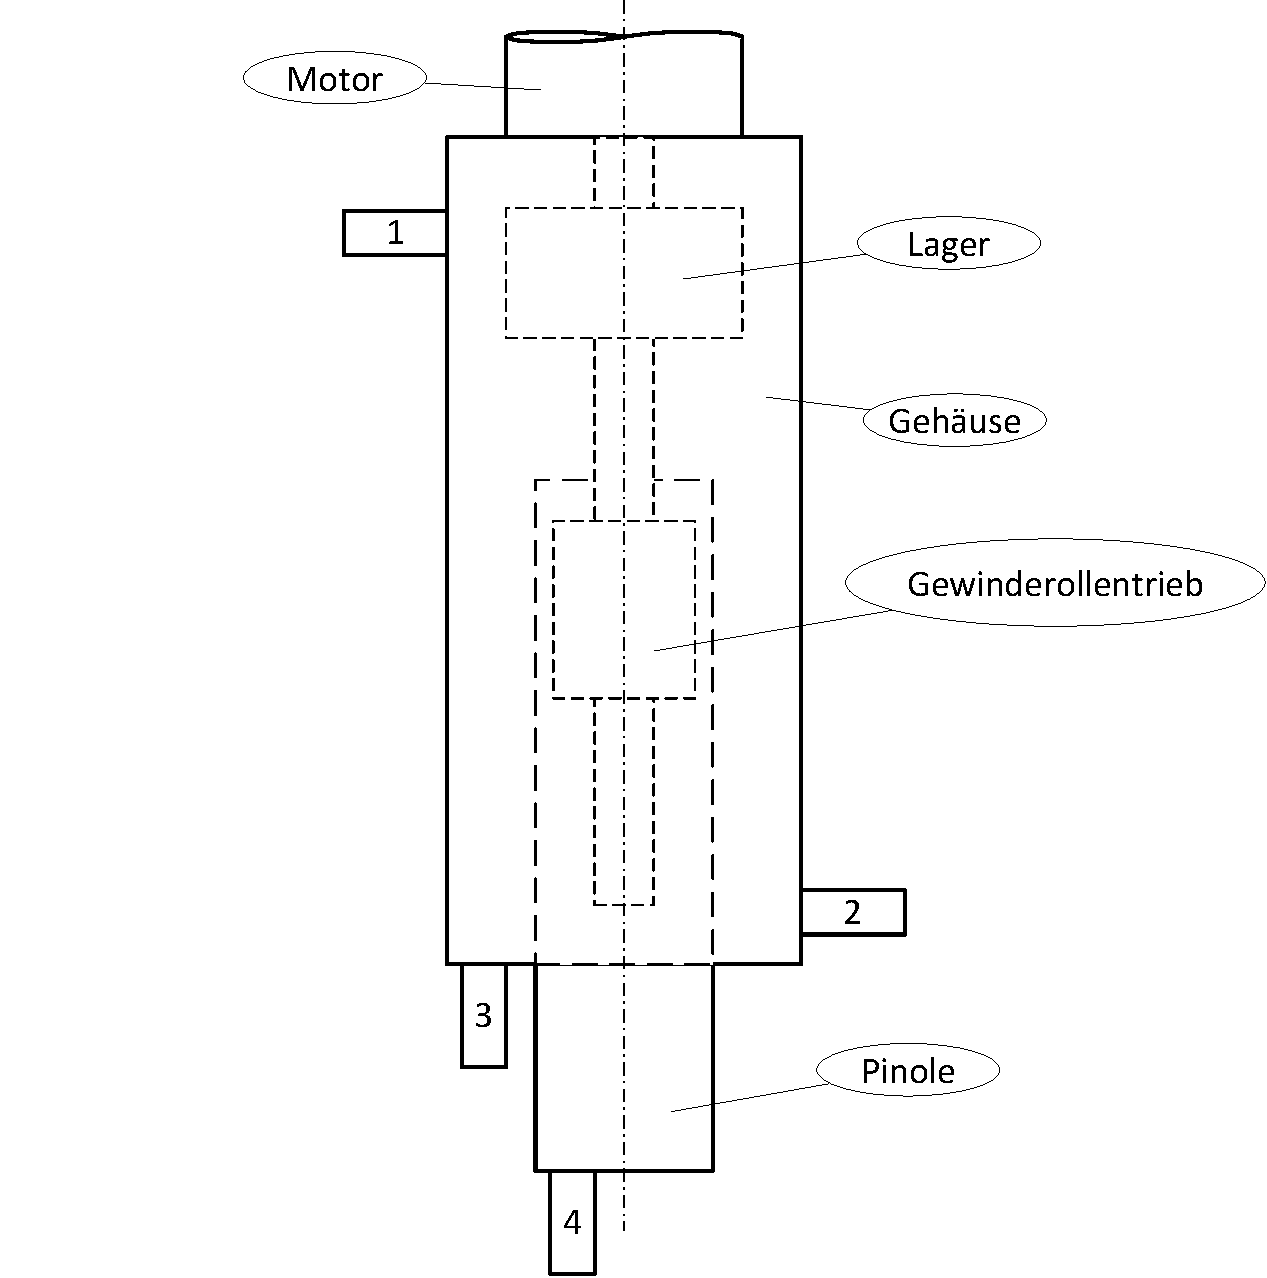
\includegraphics[height=0.5\textheight]{Positionen_Schwingungsmessung.pdf}
\caption{Position der Schwingungssensoren am NCA 5}
\label{fig:Position_der_Schwingungssensoren_am_NCA}
\end{figure}

\subsection{Auswertung der Schwingungsmessungen}

Exemplarisch werden einige Ergebnisse dargestellt, die zeigen, welche Frequenzen von bestimmten Sensoren erfasst werden konnten.




\begin{figure}[H]
\centering


\begin{tikzpicture}
 \begin{axis}[
 	no markers,
 	ymin=0,
 	%ymax=60,
    xmin=0,
    xmax=162,
 	width=\textwidth,height=0.3\textheight,
  	%title=Einfahrzyklus Drehmomentprofil,
    xlabel={Frequenz in \si{\hertz}},
    ylabel={Beschleunigung in mg},
    grid=major,
    %legend entries={Temperatursensor 1,Temperatursensor 2,Temperatursensor 3},
    %legend pos=south east,
    %enlarge x limits=0.01,
]
 	\addplot table[x=Hertz, y=mg]  {graphen/CSV_Daten/Schwingungsmessung_200mm_Seonsor1_HFFT_0,2_0-160.txt};
 	\draw(current axis.south-|{axis cs:76,1})%
       --(current axis.north-|{axis cs:76,1})node[left,pos=0.7]{Wälzkörper 76 Hz};
    \draw(current axis.south-|{axis cs:89,1})%
       --(current axis.north-|{axis cs:89,1})node[right,pos=0.7]{89 Hz Aussenring};
    \draw(current axis.south-|{axis cs:131,1})%
       --(current axis.north-|{axis cs:131,1})node[right,pos=0.7,align=left]{131 Hz \\ Innenring};
 \end{axis}
\end{tikzpicture}
\caption{Sensor 1 bei Versuch 1 und den Schadensfrequenzen des Lagers im HFFT-Spektrum}
\label{fig:Sensor_1_bei_Versuch_1_und_den_Frequenzen_des_Lagers_im_HFFT_Spektrum}
\end{figure}

In Abbildung~\ref{fig:Sensor_1_bei_Versuch_1_und_den_Frequenzen_des_Lagers_im_HFFT_Spektrum} ist die Frequenz bei Versuch 1 und dem Sensor 1 bei einer Auflösung von \SI{0.2}{\hertz} zu sehen. Es sind die Schadensfrequenzen durch das Schrägkugellager eingezeichnet. Die Frequenz des Innenrings (\SI{131}{\hertz}) ist sehr schwach zu erkennen.

\begin{figure}[H]
\centering



\begin{tikzpicture}
 \begin{axis}[
 	no markers,
 	ymin=0,
 	%ymax=60,
    xmin=0,
    xmax=10364,
 	width=\textwidth,height=0.3\textheight,
  	%title=Einfahrzyklus Drehmomentprofil,
    xlabel={Frequenz in \si{\kilo\hertz}},
    ylabel={Beschleunigung in mg},
    grid=major,
    %legend entries={Temperatursensor 1,Temperatursensor 2,Temperatursensor 3},
    %legend pos=south east,
    %enlarge x limits=0.01,
    xticklabel={\pgfmathparse{\tick/1000}\pgfmathprintnumber{\pgfmathresult}},
    scaled x ticks = false
]
 	\addplot table[x=Frequenz, y=mg]  {graphen/CSV_Daten/Schwingungssensor_200mm_Sensor1_FFT_12_0-10000.txt};
 \end{axis}
\end{tikzpicture}
\caption{Sensor 1 bei Versuch 1 FFT-Spektrum}
\label{fig:Sensor 1 bei Versuch 1 FFT Spektrum}
\end{figure}

In Abbildung~\ref{fig:Sensor 1 bei Versuch 1 FFT Spektrum} ist bei Versuch 1 mit dem Sensor 1 bei einer Auflösung von \SI{12}{\hertz} das Versuchsergebnis dargestellt.  Die Frequenz \SI{10}{\kilo\hertz} im FFT-Spektrum wird durch den Stromregler verursacht. Dies kann den Informationen über den Acopos Regler entnommen werden. \cite{BundR2007}


\begin{figure}[H]
\centering
\begin{tikzpicture}
 \begin{axis}[
 	no markers,
 	ymin=0,
    xmin=0,
    xmax=162,
 	width=\textwidth,height=0.3\textheight,
  	%title=Einfahrzyklus Drehmomentprofil,
    xlabel={Frequenz in \si{\hertz}},
    ylabel={Beschleunigung in mg},
    grid=major,
    %legend entries={Temperatursensor 1,Temperatursensor 2,Temperatursensor 3},
    %legend pos=south east,
    %enlarge x limits=0.01,
]
 	\addplot table[x=Zeit, y=mg]  {graphen/CSV_Daten/Schwingungsmessung_200mm_Sensor4_FFT_0,2_0-160.txt};
 \end{axis}
\end{tikzpicture}
\caption{Versuch 1 Sensor 4 Auflösung \SI{0,2}{\hertz} FFT-Spektrum}
\label{fig:Versuch 1 Sensor 4 Aufloesung}
\end{figure}

Aus Abbildung~\ref{fig:Versuch 1 Sensor 4 Aufloesung} ist das in Versuch 1 mit Sensor 4  gemessene FFT-Spektrum zu entnehmen. Sehr deutlich ist die Umkehrung der Bewegungsrichtung der Pinole zu erkennen. Diese hat ungefähr eine Frequenz von \SI{0,95}{\hertz}. Entsprechend wird das Aggregat mit dieser Frequenz angeregt. Daneben sind auch seine harmonischen Vielfachen zu sehen. Die sich ergebende abklingende Sinuskurve dieser Frequenz ist auf das annähernde Rechtecksignal der Beschleunigung durch das Aggregat zurückzuführen. (vgl. \cite{schnorrenberg1990spektrumanalyse})


Da keine beschädigten Bauteile für die Messungen zur Verfügung standen, konnte nicht überprüft werden, ob die in Kapitel~\ref{cha:Berechnung von Schwingungsfrequenzen} errechneten Schadensfrequenzen (vgl. Tabelle~\ref{tab:Uebersicht_Frequenzen_Schwingungsmessung}) auch bei entsprechenden Messungen festgestellt werden können.

 


\section{Temperaturmessung}




\subsection{Messung der Motortemperatur}\label{cha:Messung_der_Motortemperatur}


Der Motor besitzt einen eingebauten Temperatursensor. Die Motortemperatur wird durch die Steuerung der Maschine ausgelesen und dient dort, falls gewünscht, zur Thermokompensation von NCAs. Mit der Thermokompensation kann die temperaturbedingte Längen- oder Wegveränderung an den NCAs durch die Steuerung ausgeglichen werden (vgl. \cite{OttoBihlerMaschinenfabrikGmbH&Co.KG2015}). Die Erfassung der Motortemperatur im bisherigen Testablauf wird in Kapitel~\ref{cha:Einlaufen_Motortemperatur} beschrieben.





% ist ein sehr guter Indikator, ob die Achse thermisch ausgelastet ist. Bei zu geringer Kühlung durch das Kühlmittel kann die Achse nicht mehr genügend gekühlt werden. durch eine unnormmal hohe Temperatur kann ein Problem im Kühlkreislauf festgestellt werden.

Die Motortemperatur ist ein sehr guter Indikator, in wie weit die Achse bis an die Leistungsgrenze belastet wird. Je höher die Motorleistung ist, desto höher wird die Motortemperatur. Um möglichst hohe Kräfte mit einem bestimmten NCA zu erzeugen, ist in die NCAs ein Kühlkreislauf, wie in Kapitel~\ref{cha:Kuelkreislauf_Schmierkreislauf} erwähnt, eingebaut.  Bei zu geringer Kühlung durch das Kühlmittel kann die Achse nicht mehr genügend gekühlt werden. Die Motortemperatur steigt dann an.






Eine über den Normbereich hinausgehende Temperatur kann nicht nur auf ein Problem mit dem Motor hinweisen, sondern aufgrund der Kühlung auch auf ein eventuelles Problem im Kühlkreislauf. Probleme, die mit dem Kühlkreisaluf zusammenhängen, sind in Kapitel~\ref{cha:Durchflussmessung_Kühlwasser} näher erläutert. Für die Messung ist interessant, dass bei mangelnder Kühlung die Temperatur um so stärker ansteigt je mehr die Achse belastet wird. Eine hohe Belastung der Achse steigert die Aussagekraft der Messung der Motortemperatur. Je höherer die Achse belastet wird, desto eher kann man anhand der Analyse der Temperaturwerte feststellen, ob es Probleme mit dem Kühlkreislauf gibt.



Leider konnten keine aussagekräftigen Werte für die Motortemperatur ermittelt werden, da diese in der Steuerung der VC 1 nur als Momentanwert angezeigt werden und nicht aufgezeichnet und gespeichert werden können. Grundsätzlich ist die Erfassung der Motortemperatur sinnvoll, aber der Aufwand, um ein funktionierendes System zu etablieren, das die erfassten Daten entsprechend auswerten kann, ist zu groß. 



\subsection{Messung der Temperatur mit externen Sensoren}

Wie bereits bei dem jetzigen Testablauf beschrieben (vgl. Kapitel~\ref{cha:Temperatur_an_der_Aussenseite_des_NCA}), wird die Temperatur an der Außenseite des Aggregates durch Temperatursensoren gemessen. Wie bereits in Kapitel~\ref{ch:Kritik_Testlauf} erwähnt, ist die Aussagekraft dieser Messung als gering einzuschätzen. Der Aufwand dieser Messung ist zu groß im Verhältnis zum Nutzen, um diese Messung sinnvoll in der Serienmessung einzusetzen.

% Kühlwassertemperatur

Eigentlich wäre die Temperatur im Inneren der Achse, hier insbesondere auf der Spindel des Gewinderollentriebes, von Interesse. Somit könnten Probleme des Gewinderollentriebes erkannt werden. Allerdings steht auch hier der Aufwand zum Nutzen in keinem ökonomisch vertretbaren Verhältnis.




\section{Volumenstrommessung}

Um das Aggregat dauerhaft zu betreiben, muss die Versorgung mit Kühlwasser und Schmieröl gesichert sein. Um festzustellen, ob diese Versorgung fehlerfrei abläuft, bietet sich eine Messung der Durchflussrate bzw. des Volumenstromes der beiden Medien an.





\subsection{Volumenstrommessung des Kühlwassers}\label{cha:Durchflussmessung_Kühlwasser}



Wie in Kapitel~\ref{cha:Messung_der_Motortemperatur} zu sehen, hängen Kühlmitteldurchfluss und Motortemperatur sehr eng zusammen. So steigt die Motortemperatur bei hoher Belastung der Achse, bei Problemen mit dem Motor, aber auch bei Problemen mit dem Kühlmittelkreislauf. Wenn der Kühlmittelkreislauf funktioniert, kann er die Temperaturanstiege kompensieren.

Als Grund für eine zu geringe Kühlung kommt häufig ein zu geringer Durchsatz an Kühlmittel in Frage. Der zu geringe Durchsatz kann verschiedene Ursachen haben.  Zum einen kann es Probleme im Kühlkreislauf außerhalb des Aggregates geben. Zum anderen können die Probleme auch innerhalb des NCAs auftreten. Dabei kommt es immer wieder zu Verstopfungen innerhalb des NCAs, die den Kühlmitteldurchfluss verringern. Derartige Verstopfungen werden bei neuen NCAs z.B. durch Späne oder sonstige Gegenstände wie z.B. Dichtstopfen hervorgerufen. Diese Probleme werden unter anderem durch unsachgemäße Montage und nicht entfernte Späne verursacht.



Die Größen Volumenstrom $Q$ und die Druckdifferenz $\Delta p = p_1 - p_2$ sind messtechnisch mit den entsprechenden Messinstrumenten relativ leicht automatisiert zu erfassen. Die Dichte des Kühlmittels beträgt: $\rho = \SI{1041}{\kilogram\per\liter} $ bei \SI{20}{\degreeCelsius}. Als Kühlmittel wird ein Antifrogen-N Wassergemisch der Firma Westfalen AG mit 30 Vol.\% verwendet.


\begin{figure}[h]
\centering
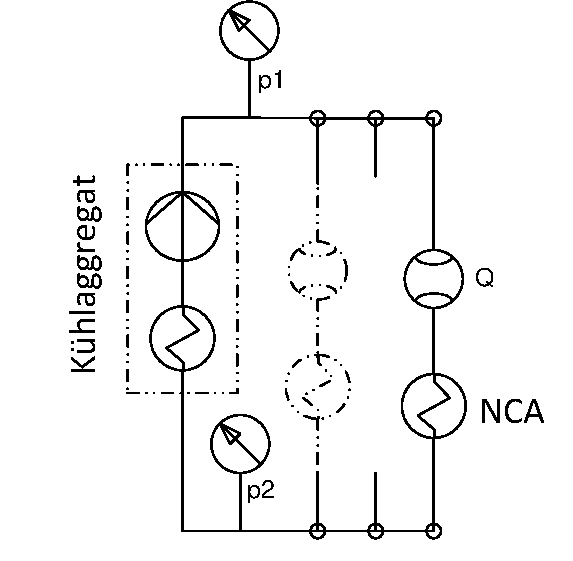
\includegraphics[width=0.5\textwidth]{Kuehlkreislauf_Skizze.pdf} 
\caption{Schematische Darstellung des Kühlkreislaufs mit den Messpunkten $p_1$, $p_2$ und $Q$ } 
\label{fig:Kuehlkreislauf_Skizze}
\end{figure}


Nach dem Ende des Testlaufs wird in Ruhestellung bei jedem einzeln der NCAs nacheinander der Kühlmitteldurchfluss gemessen, wobei sie noch im Prüfstand aufgehängt sind. Die Anordnung der Messpunkte ist der Abbildung~\ref{fig:Kuehlkreislauf_Skizze} zu entnehmen.

Zur Messung des Volumenstroms bzw. der Kühlmitteldurchflussrate wird das Messgerät e8611 mit dem Aufsatz Typ S030 HT der Firma Bürkert verwendet.

Zum Vergleich der erfassten Werte bietet sich die Bildung einer Kennzahl an. Dafür eignet sich in diesem Fall der $k_\mathrm{v}$ Wert (vgl. \cite{Glueck1988}).

\begin{equation}
 k_\mathrm{v} = Q \cdot  \sqrt{\frac{\rho }{\Delta p}}
\end{equation}

Physikalisch ist unter $k_\mathrm{v}$ eine verminderte Durchströmfläche zu verstehen. Der geometrisch kleinste Querschnitt wird durch Strahleinschnürung und Wirbelbildung noch weiter verringert.

% Der hier verwendete $k_\mathrm{v}$ Wert ist der physikalisch korrekte Kennwert und nicht der in der VDI / VDE Richlinie 2173 \cite{verband1962vdi} definierte $K_v$ Wert in \si{\cubic\meter\per\hour}. 

Hier wird der $k_\mathrm{v}$ Wert über die SI Einheiten berechnet. Alternativ gibt es noch den weit verbreiteten $K_v$ Wert in \si{\cubic\meter\per\hour} (vgl. die VDI / VDE Richtlinie 2173 \cite{verband1962vdi}). Dieser ist allerdings physikalisch nicht korrekt, da es sich hierbei um eine zugeschnittene Größengleichung handelt (vgl. \cite{Glueck1988}). 


Alternativ kann auch der wesentlich bekanntere und verbreitetere  Druckverlustbeiwert $\zeta$ verwendet werden. Die Umrechnung von $k_\mathrm{v}$ auf $\zeta$ kann der Gleichung~\ref{eq:Druckverlustbeiwert} entnommen werden: 

\begin{equation}\label{eq:Druckverlustbeiwert}
\zeta = 2 \cdot \frac{ A^2}{ {k_\mathrm{v}}^2}
\end{equation}

$A$ entspricht dem kleinsten Querschnitt innerhalb des Kühlkreislaufes des Aggregates. Hier kann der laut Konstruktionszeichnung kleinste vorgesehene Querschnitt genommen werden.

In der Tabelle~\ref{tab:Durchflussmessung_Kuehlung} sind die gemessenen Durchfluss- und Druckwerte und die daraus berechneten Kennzahlen aufgeführt.


\begin{table}[h]
\centering




\begin{tabular}{cccccccc}\toprule
Seriennummer & NCA & Datum & Zustand & $Q$ & $p_1$ & $p_2$ & $k_\mathrm{v}$ \\
 &  &  &  & L / min & bar & bar & \si{\milli\meter\squared} \\ 
 \midrule
38094 & NCA 5 & 22.05.2015 & neu & 2,08 & 3,6 & 1 & 2,19 \\
38095 & NCA 5 & 22.05.2015 & neu & 1,93 & 3,6 & 1 & 2,04 \\
38163 & NCA4 & 12.06.2015 & neu & 1,95 & 3,75 & 1 & 2,00 \\
38164 & NCA4 & 12.06.2015 & neu & 1,91 & 3,75 & 1 & 1,96 \\
38177 & NCA4 & 12.06.2015 & neu & 1,92 & 3,75 & 1 & 1,97 \\
38162 & NCA4 & 12.06.2015 & neu & 1,98 & 3,75 & 1 & 2,03 \\
38168 & NCA4 & 15.06.2015 & neu & 1,98 & 3,5 & 1 & 2,13 \\
38179 & NCA4 & 15.06.2015 & neu & 2,01 & 3,5 & 1 & 2,16 \\
38174 & NCA4 & 15.06.2015 & neu & 2,05 & 3,5 & 1 & 2,20 \\
38172 & NCA4 & 15.06.2015 & neu & 2 & 3,5 & 1 & 2,15 \\
38171 & NCA4 & 16.06.2015 & neu & 1,92 & 3,1 & 1 & 2,25 \\
38173 & NCA4 & 16.06.2015 & neu & 1,87 & 3,1 & 1 & 2,19 \\
38167 & NCA4 & 16.06.2015 & neu & 1,9 & 3,1 & 1 & 2,23 \\
\bottomrule
\end{tabular}




\caption{Gemessene Werte Volumenstrom Kühlflüssigkeit}
\label{tab:Durchflussmessung_Kuehlung}
\end{table}


Die $k_v$ Werte der gemessenen NCA 4 besitzen einen Mittelwert von \SI{2,115}{\milli\meter\squared} und eine Standardabweichung von \SI{0,101}{\milli\meter\squared}. Um zu einer höheren statistischen Sicherheit zu gelangen, sollten weitere Messungen erfolgen. Als Eingriffsgrenzen bieten sich die Abweichungen von $\pm 2\sigma$ vom empirischen Mittelwert an. Dies ergibt bei dem derzeitigen Stichprobenumfang eine untere Eingriffsgrenze von \SI{1,913}{\milli\meter\squared} und eine obere Eingriffsgrenze von \SI{2,317}{\milli\meter\squared}. Alle der bis jetzt getesteten Achsen befinden sich innerhalb dieses Intervalls.

Ein Vorteil der Durchflussmessung ist neben der Analyse der neuen NCAs auch, dass bei entsprechend systematischer Erfassung und Aufzeichnung der Werte für später zu untersuchende Rückläufer aus Reklamationen Referenzwerte zur Verfügung stehen.

\subsection{Volumenstrommessung des Schmieröls }

Da die in Kapitel~\ref{cha:Kuelkreislauf_Schmierkreislauf} beschriebene Schmiermittelversorgung für die Funktionsfähigkeit der NCAs elementar ist, ist es wichtig festzustellen, ob sie zuverlässig funktioniert. Auch hier kann wie bei der Kühlmittelversorgung eine Volumenstrommessung in Erwägung gezogen werden. Damit könnte man feststellen, ob die Zumessventile zuverlässig die erforderliche Menge Schmierstoff zudosieren. Eine Messung gestaltet sich allerdings durch den geringen und impulsförmigen Durchsatz als schwierig. Die Erfahrungen mit der Verwendung der Zumessventile zeigen, dass diese im Allgemeinen zuverlässig funktionieren und somit der Aufwand durch die Volumenstrommessung des Schmieröls in der Serienfertigung nicht gerechtfertigt ist. 

Zudem wäre die Verteilung des Schmiermittels im Innern des Aggregates eine aussagekräftigere Messgröße.  Dies kann allerdings, falls überhaupt, nur mit großem Aufwand (z.B. Demontage des Aggregates) gemessen werden.




\section{Messung der Bremshaltekraft}\label{cha_Messung_der_Bremshaltekraft}



In der Abteilung Versuch wird bei der Erstbemusterung, den ausführlichen Tests an einem Prototyp der NCAs, die Haltekraft der Bremse des Motors getestet. Die Motorbremse dient dazu, die Achse in ihrer Position zu halten, wenn der Motor stromlos ist. Dazu wird, wie in Abbildung~\ref{fig:Darstellung_Bremshaltekraft_bestimmen} zu sehen, ein Hydraulikzylinder mit montiertem Kraftsensor unter die stromlose Achse gestellt. Nun wird der Hydraulikzylinder ausgefahren, so dass er gegen die Achse drückt, so lange bis die Bremse nachgibt. Dabei wird die maximale Kraft gemessen, die die Achse halten kann. 

\begin{figure}[H]
\centering
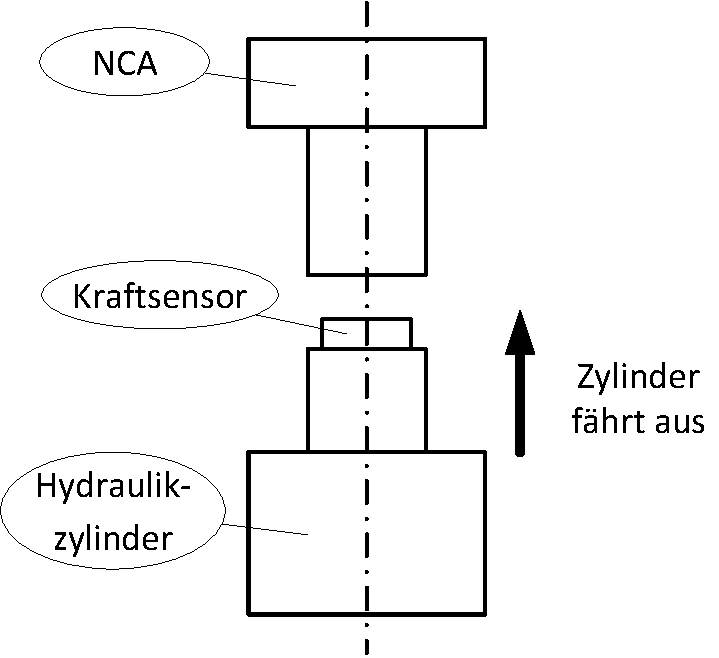
\includegraphics[width=0.5\textwidth]{Bremshaltekraft_Bestimmen} 
\caption{Schema des Versuchsaufbaus zur Bestimmung der Bremshaltekraft} 
\label{fig:Darstellung_Bremshaltekraft_bestimmen}
\end{figure}

% Da es mit den Haltebremsen bis jetzt keine größeren Probleme gab ist es derzeit nicht sinnvoll diesen aufwendigen Test für die NCAs in der Serienfertigung zu verwenden.

Dieser Test ist sehr aufwendig. Da die Haltebremsen bis jetzt meist zuverlässig funktionieren, erscheint es nicht sinnvoll, ihn in der Serienfertigung einzusetzen.















%\section{Inbetriebnahme}

% Nachdem die NCAs montiert sind, was bedeutet, dass die Montage der NCAs grundsätzlich funktioniert hat, werden sie zum Einlaufen und Testen im derzeitigen Testverlauf an den Prüfstand angebaut (Kapitel~\ref{cha:Beschreibung_des_Testablaufs}). Danach werden sie an die Steuerung angeschlossen, um sie betreiben zu können. Diese Inbetriebnahme ist ein grundlegender Test, wie in Kapitel~\ref{cha_Tests_in_der_Versuchsabteilung} ausgeführt, der in jeden Prüfverlauf eingebaut werden muss, denn er zeigt, dass das Zusammenspiel von Achse und Steuerung funktioniert. Somit zeigt der Test der Inbetriebnahme, dass ein Betreiben der NCAs möglich.